\documentclass{tufte-handout}\usepackage[]{graphicx}\usepackage[]{color}
% maxwidth is the original width if it is less than linewidth
% otherwise use linewidth (to make sure the graphics do not exceed the margin)
\makeatletter
\def\maxwidth{ %
  \ifdim\Gin@nat@width>\linewidth
    \linewidth
  \else
    \Gin@nat@width
  \fi
}
\makeatother

\definecolor{fgcolor}{rgb}{0.345, 0.345, 0.345}
\makeatletter
\@ifundefined{AddToHook}{}{\AddToHook{package/xcolor/after}{\definecolor{fgcolor}{rgb}{0.345, 0.345, 0.345}}}
\makeatother
\newcommand{\hlnum}[1]{\textcolor[rgb]{0.686,0.059,0.569}{#1}}%
\newcommand{\hlstr}[1]{\textcolor[rgb]{0.192,0.494,0.8}{#1}}%
\newcommand{\hlcom}[1]{\textcolor[rgb]{0.678,0.584,0.686}{\textit{#1}}}%
\newcommand{\hlopt}[1]{\textcolor[rgb]{0,0,0}{#1}}%
\newcommand{\hlstd}[1]{\textcolor[rgb]{0.345,0.345,0.345}{#1}}%
\newcommand{\hlkwa}[1]{\textcolor[rgb]{0.161,0.373,0.58}{\textbf{#1}}}%
\newcommand{\hlkwb}[1]{\textcolor[rgb]{0.69,0.353,0.396}{#1}}%
\newcommand{\hlkwc}[1]{\textcolor[rgb]{0.333,0.667,0.333}{#1}}%
\newcommand{\hlkwd}[1]{\textcolor[rgb]{0.737,0.353,0.396}{\textbf{#1}}}%
\let\hlipl\hlkwb

\usepackage{framed}
\makeatletter
\newenvironment{kframe}{%
 \def\at@end@of@kframe{}%
 \ifinner\ifhmode%
  \def\at@end@of@kframe{\end{minipage}}%
  \begin{minipage}{\columnwidth}%
 \fi\fi%
 \def\FrameCommand##1{\hskip\@totalleftmargin \hskip-\fboxsep
 \colorbox{shadecolor}{##1}\hskip-\fboxsep
     % There is no \\@totalrightmargin, so:
     \hskip-\linewidth \hskip-\@totalleftmargin \hskip\columnwidth}%
 \MakeFramed {\advance\hsize-\width
   \@totalleftmargin\z@ \linewidth\hsize
   \@setminipage}}%
 {\par\unskip\endMakeFramed%
 \at@end@of@kframe}
\makeatother

\definecolor{shadecolor}{rgb}{.97, .97, .97}
\definecolor{messagecolor}{rgb}{0, 0, 0}
\definecolor{warningcolor}{rgb}{1, 0, 1}
\definecolor{errorcolor}{rgb}{1, 0, 0}
\makeatletter
\@ifundefined{AddToHook}{}{\AddToHook{package/xcolor/after}{
\definecolor{shadecolor}{rgb}{.97, .97, .97}
\definecolor{messagecolor}{rgb}{0, 0, 0}
\definecolor{warningcolor}{rgb}{1, 0, 1}
\definecolor{errorcolor}{rgb}{1, 0, 0}
}}
\makeatother
\newenvironment{knitrout}{}{} % an empty environment to be redefined in TeX

\usepackage{alltt}

%\geometry{showframe}% for debugging purposes -- displays the margins

\usepackage{amsmath}
\usepackage{natbib}
\bibfont{\small} % Doesn't see to work...

% Set up the images/graphics package
\usepackage{graphicx}
\setkeys{Gin}{width=\linewidth,totalheight=\textheight,keepaspectratio}
% \graphicspath{{graphics/}}
\title{Overview of R %\thanks{}
}
\author[Marc Los Huertos]{Marc Los Huertos}
\date{}  % if the \date{} command is left out, the current date will be used


% \SweaveOpts{prefix.string=graphics/plot} % Created a "graphics" subdirectory to 

\setsidenotefont{\color{blue}}
% \setcaptionfont{hfont commandsi}
% \setmarginnotefont{\color{blue}}
% \setcitationfont{\color{gray}}

% The following package makes prettier tables.  We're all about the bling!
\usepackage{booktabs}

% Small sections of multiple columns
\usepackage{multicol}

% These commands are used to pretty-print LaTeX commands
% command name -- adds backslash automatically
\newcommand{\docpkg}[1]{\texttt{#1}}% package name
\newcommand{\doccls}[1]{\texttt{#1}}% document class name
\newcommand{\docclsopt}[1]{\texttt{#1}}% document class option name
\IfFileExists{upquote.sty}{\usepackage{upquote}}{}
\begin{document}

\maketitle% this prints the handout title, author, and date
\begin{abstract}
\noindent R is a robust, open source software package to process and analyzed data. As an extremely flexible programming environment, its development has been rapid and popularity has been growing dramatically in recent years. Most graduate schools teach R and many are phasing out the traditional software package site licenses (\eg SAS, SPSS, etc). 

This handout provides an brief introduction to the syntax of R and some applications to plot and bivariate data. I believe R provides a mechanism to learn 1) skills to process electronic data, 2) a programming environment to implement a range of statistical tests, and 3) provide skills that can be used in your future career, whether or not R is used again.\sidenote{Typeset using the Sweave function in R and \LaTeX\ using a \citet{Tufte:1983, Tufte:1997} and style.}
\end{abstract}

%\printclassoptions

% Setting up the margins, etc for R


\section{Session Outcomes}
\begin{enumerate}
	\item Open and use the R GUI with consistent results.
	\item Use math operators to solve simple calculations.
	\item Create objects.
	\item Solve repetitive calculations.
	\item Make a function.
	\item Get data into the R environment.
	\item Generate summary statistics.
	\item Build and test a linear model.
	\item Create publication quality graphics.
\end{enumerate}

\section{The R GUI}

Starting the program is fairly easy.\sidenote[][-.5in]{Outcome: Open R and use the R GUI with consistent results.} Assuming R is installed,\footnote[][.03in]{If R is not installed, it can be done easily by going to http://www.r-project.org/ and downloading the free software "base" program, which have been compiled for Windows and Mac and there is source code for Linux and Unix boxes.} find R by going to the windows "Start" button, navigate to "All Programs" and search for "R". Click on R program, whose icon is usually an capital R followed by a version number. 

Now that R is started, you should notice a few things.  The GUI, or graphical user interface is quite Spartican, compared to what computers are capable of. For beginners this is the most disturbing part of the program. Second, there are some hints of how to start, but to follow these hints, you have to type exactly what you see. Yes, computers are stupid, they only recognized the commands they expect, not what you want them to understand. 

\begin{figure}
		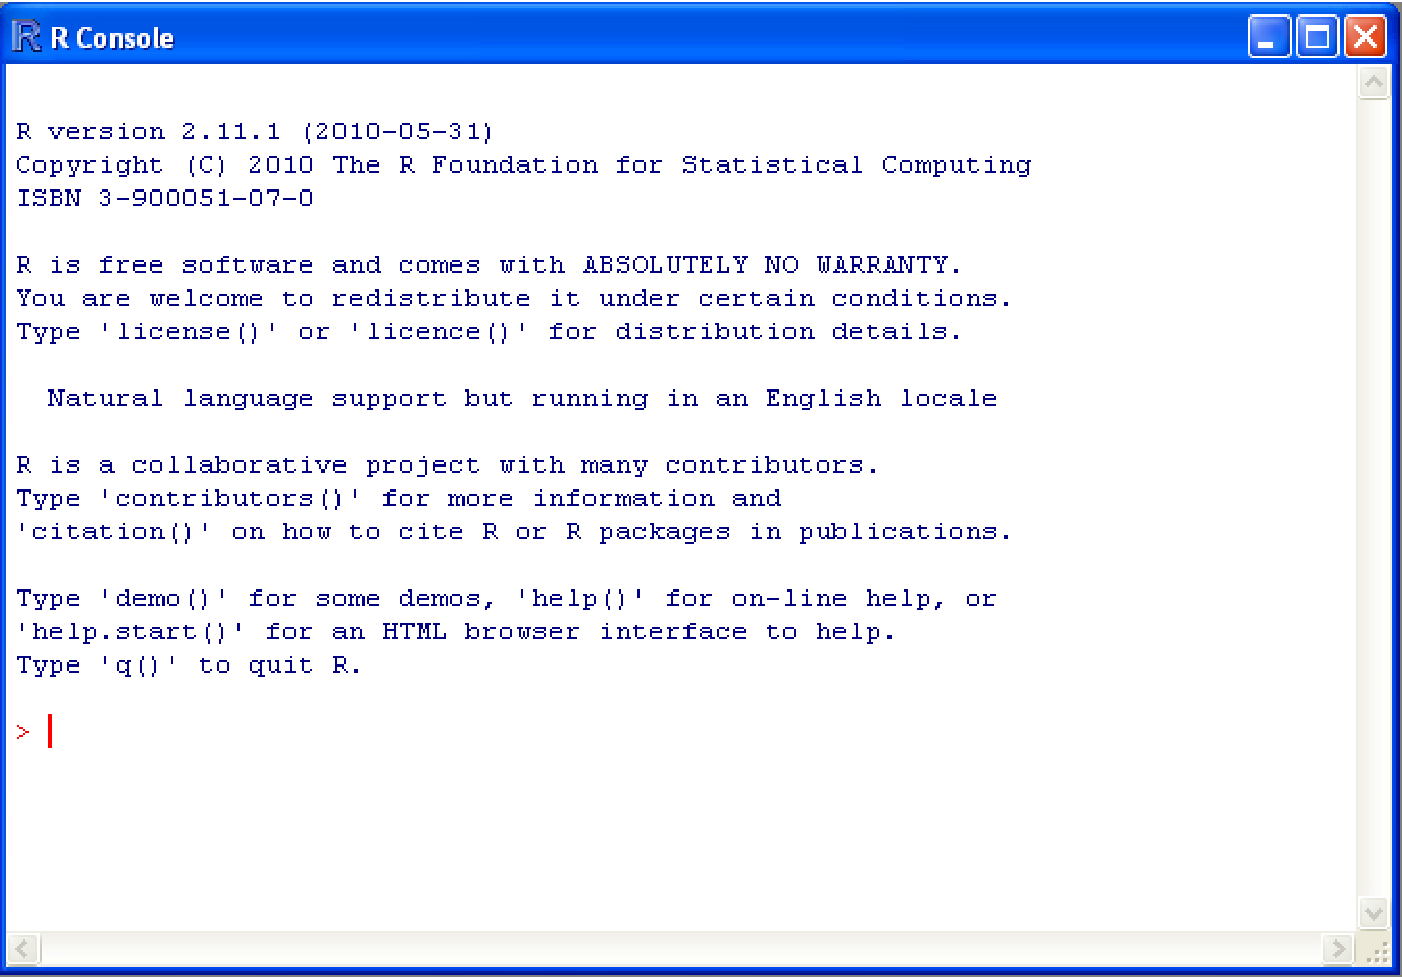
\includegraphics{OpeningScreenShot.pdf}
	\caption{Opening window screen shot of R. Notice the version number is probably different than what you have. Don't worry about this, the differences are minor and only play a significant role as you start to do more advanced statistics. There are new versions every few months and I might be a few versions ahead or behind what you see. Also, notice some hints have been created for the beginner. However, you much type exactly what you see including the parentheses. Most commands in R have parentheses, which signifies a function, which are like verbs in R. Without a function (or verb), R doesn't really know what to do.}
	\label{fig:OpeningScreenShot}
\end{figure}

At the bottom of the screen is a prompt, which is a ">" symbol. Yes, you could change that to something more recognizable, but later you will appreciate the simplicity. This is where R expects commands lines to be entered. This characteristic is why R is called a command line program. There are no buttons to push and the menus are pretty limited.
  
Let's start with closing R.  Type "quit()" to close R. Notice that R asked you to save the workspace. R keeps track of your typing history and objects that you create. I'll explain objects soon enough. I generally don't save anything, if you do, you might find a bewildering number of objects that will interfere with your work at a later date. So, click "no" and R goes away.

Start R again. Congratulations, you have just met the first outcome. You can smile and get a drink of water.

Before moving on, open a word processor and begin recording your response to following question and question at the end of each section.

\bigskip
\noindent \textbf{\#1 Please list three or four questions you have so far. }

\section{R as a Calculator}

Using a computer for calculating values has become a trivial exercise with the widespread use of Excel.\sidenote{Outcome: Use math operators to solve simple calculations.} However, there are a number of symbols required when you are doing math functions on a computer because the keyboard is not specialized like a calculator. Thus, we have to learn how to use operators using simple keyboard characters. See the Table~\ref{tab:KeyboardOperators} for a list of the common characters used for operators in R.

\begin{table}
	\begin{center}
	\begin{tabular}{lcc}
		\toprule
Operation &\ Operator &\ Example \\
\midrule
Addition & + &  6 + 5  \\  
Subtraction & - & 6 - 5 \\
Multiplication & * & 6 * 5 \\
Division & / & 3 / 5\\
Power & $\wedge$ & 3 $\wedge$ 5  \\
\bottomrule
\end{tabular}
\end{center}	
\caption{Keyboard Operator for Mathematical Operations in R.}
	\label{tab:KeyboardOperators}
\end{table}

In addition, for more complex operations, R uses functions, which have a different syntax, \eg \texttt{log()}, \texttt{exp()}, \texttt{sin()}, etc. The syntax for these functions is fairly straightforward. For example, to calculate the base 10 logarithm of 3.5, we can type:\sidenote{as below, each time you see a ``>'', I am referring to the R prompt and you want to type the text after the prompt.}

\begin{knitrout}
\definecolor{shadecolor}{rgb}{0.969, 0.969, 0.969}\color{fgcolor}\begin{kframe}
\begin{alltt}
\hlkwd{log10}\hlstd{(}\hlnum{3.5}\hlstd{)}
\end{alltt}
\begin{verbatim}
## [1] 0.544068
\end{verbatim}
\end{kframe}
\end{knitrout}

Or to calculate the natural log, type
\begin{knitrout}
\definecolor{shadecolor}{rgb}{0.969, 0.969, 0.969}\color{fgcolor}\begin{kframe}
\begin{alltt}
\hlkwd{log}\hlstd{(}\hlnum{3.5}\hlstd{)}
\end{alltt}
\begin{verbatim}
## [1] 1.252763
\end{verbatim}
\end{kframe}
\end{knitrout}

R allows the user to make complex equations and even solving complex calculations. For example, the if you want to solve the following equation:

\begin{equation}
V = V_{max}\frac{S}{K_s + S}
\end{equation}

And $V_{max}$ = 3, $S$ = 1.0 and $K_s = 0.3$, then you can type

\begin{knitrout}
\definecolor{shadecolor}{rgb}{0.969, 0.969, 0.969}\color{fgcolor}\begin{kframe}
\begin{alltt}
\hlnum{3.0} \hlopt{*} \hlstd{(}\hlnum{1.0} \hlopt{/} \hlstd{(}\hlnum{0.3} \hlopt{+} \hlnum{1.0}\hlstd{))}
\end{alltt}
\begin{verbatim}
## [1] 2.307692
\end{verbatim}
\end{kframe}
\end{knitrout}

However, typing these formulas can be time consuming and subject to typos, (\eg it is easy to forget to put the parentheses in the right place) so we'll see how we can streamline the process to make R uses more efficient. 

\bigskip
\noindent \textbf{\#2 What are the differences between what you have seen in other computer programs so far? }

\section{Objects in R}

\subsection{Creating Objects}

Typing a long string of numbers each time you want to due something is a waste of time and effort. Let's say you wanted to have the numbers from 1 to 10. But R would have no way to handle this series. Instead, we use R to store these values in an object and recall them at will. To create objects in R, we use either the \texttt{=} or the \texttt{<-} symbols, which is composed of a ``less than symbol'' and a ``dash.'' I prefer the second because it is obviously directional and thus there is no ambiguity.\sidenote{Outcome: Create Objects.}

When creating an object, we need to name the object and define the object type. Usually, this can be done in a single step. But we'll try to break it down so you can follow along. First, let's say we want to make an object that has 10 numbers in it. The most basic type of object is a vector, which can store a string of numbers or characters. Let's call the vector something recognizable, \texttt{myvector}. To put numbers into a vector, we need to concatenate or combine them, thus we need R to do something with the numbers, in other words, we need a "verb". In this case the verb concatenate or combine is abbreviated as \texttt{c()}. Remember with each function, there are parentheses. Now what we put ten numbers into the parentheses to be concatenated. We'll put a series of numbers from 1 to 10. 

\begin{knitrout}
\definecolor{shadecolor}{rgb}{0.969, 0.969, 0.969}\color{fgcolor}\begin{kframe}
\begin{alltt}
\hlstd{myvector} \hlkwb{<-} \hlkwd{c}\hlstd{(}\hlnum{1}\hlstd{,} \hlnum{2}\hlstd{,} \hlnum{3}\hlstd{,} \hlnum{4}\hlstd{,} \hlnum{5}\hlstd{,} \hlnum{6}\hlstd{,} \hlnum{7}\hlstd{,} \hlnum{8}\hlstd{,} \hlnum{9}\hlstd{,} \hlnum{10}\hlstd{)}
\end{alltt}
\end{kframe}
\end{knitrout}

In this case, each number to be combined is separated by a comma. Spaces between the commas does not affect the object at all. Notice when you create the vector, R does not return any response. At first, this might seem disconcerting. But soon, you will be excited by the silence. In general, no news is good news in R, i.e. when there is no response, R did something and there was no error. Now it might not be what you wanted, but it did something. So, now let's see if R did what we wanted. 

Now, we can view the vector by typing the name of the vector as below:\sidenote{The numbers in the square brackets are referencing the "index" number of the first observation in the row. It will make more sense when we create longer vectors.}  

\begin{knitrout}
\definecolor{shadecolor}{rgb}{0.969, 0.969, 0.969}\color{fgcolor}\begin{kframe}
\begin{alltt}
\hlstd{myvector}
\end{alltt}
\begin{verbatim}
##  [1]  1  2  3  4  5  6  7  8  9 10
\end{verbatim}
\end{kframe}
\end{knitrout}

\subsection{Interrogating Objects}

We now use a function to interrogate the vector. For example, how long is the vector?

\begin{knitrout}
\definecolor{shadecolor}{rgb}{0.969, 0.969, 0.969}\color{fgcolor}\begin{kframe}
\begin{alltt}
\hlkwd{length}\hlstd{(myvector)}
\end{alltt}
\begin{verbatim}
## [1] 10
\end{verbatim}
\end{kframe}
\end{knitrout}

What is the sum of the values in the vector?

\begin{knitrout}
\definecolor{shadecolor}{rgb}{0.969, 0.969, 0.969}\color{fgcolor}\begin{kframe}
\begin{alltt}
\hlkwd{sum}\hlstd{(myvector)}
\end{alltt}
\begin{verbatim}
## [1] 55
\end{verbatim}
\end{kframe}
\end{knitrout}

What is the mean of the vector?

\begin{knitrout}
\definecolor{shadecolor}{rgb}{0.969, 0.969, 0.969}\color{fgcolor}\begin{kframe}
\begin{alltt}
\hlkwd{mean}\hlstd{(myvector)}
\end{alltt}
\begin{verbatim}
## [1] 5.5
\end{verbatim}
\end{kframe}
\end{knitrout}

Congratulations, you have now made an object. This object is a vector, which we  named "myvector".\footnote{By the way, R is case sensitive, so "myvector" or "myVector" or "Myvector" refer to two different objects, two of which don't exists. Failing to keep track of what is upper and lower case can lead to high levels of frustration. I suggest you start with keeping everything lower case to avoid confusion. However, I will violate this suggestion immediately, for reasons that I will explain below.} Another thing to notice is that we have created a vector of numbers, would have also created a vector of characters (and words) and logical or binary responses, \ie TRUE and FALSE.

\bigskip
\noindent \textbf{\#3 Please list what questions might have come up in this section? }

\subsection{Types of Objects}

There a variety of objects that can be created in R (Table~\ref{tab:CommonObjects}). For the purpose of our class, we will concentrate on the following objects:
\begin{table}
	\centering
		\begin{tabular}{ll}
Object Type &\ Coercive functions \\
\hline
Vector & \texttt{c()}, \texttt{as.vector()} \\
Matrix & \texttt{matrix()}, \texttt{as.matrix()} \\
List & \texttt{list()}, \texttt{as.list()} \\
Data frame & \texttt{data.frame()}, \texttt{as.data.frame()} \\
Linear model & \texttt{lm()}, \texttt{aov()} \\\hline
		\end{tabular}
	\caption{Examples of common objects and the coercive functions to create them. We will use many of these, so do not worry if you don't know what they mean yet.}
	\label{tab:CommonObjects}
\end{table}

For now, we will create a data frame, which is the most common type of object for statistical analysis. A data.frame is like a spreadsheet in Excel or a table. However, it has some important unique characteristics. First, the data.frame is composed of vectors of equal length. Second, the the data frame of often described as a list of vectors. Thus, the data frame is combines the vectors in a certain way. 

Several researchers have been investigating the effects of ambient temperatures on snow melt, soil moisture and plant phenology. In a series of experiments with heaters above a few feet above the snow, researchers looked at measures several responses. For this exercise, we'll just look at two vectors to create a data frame.

There were 3 treatments and 5 replicates, for a total of 15 observations. Since vectors can be either numeric or character, we'll use characters to represent the three treatments: Heated, Control, and Procedure Control. The procedure control had heaters installed but not turned on. This tests whether there was an effect of the heaters just being present. We will coerce the data into a vector called Treatment.
For vectors, we will put the treatments names in quotes. Also to avoid having to type each treatment 5 times, will use the repeat function.


\begin{knitrout}
\definecolor{shadecolor}{rgb}{0.969, 0.969, 0.969}\color{fgcolor}\begin{kframe}
\begin{alltt}
\hlkwd{rep}\hlstd{(}\hlstr{"Control"}\hlstd{,} \hlnum{5}\hlstd{)}
\end{alltt}
\begin{verbatim}
## [1] "Control" "Control" "Control" "Control" "Control"
\end{verbatim}
\begin{alltt}
\hlkwd{rep}\hlstd{(}\hlstr{"Treatment"}\hlstd{,} \hlnum{5}\hlstd{)}
\end{alltt}
\begin{verbatim}
## [1] "Treatment" "Treatment" "Treatment" "Treatment"
## [5] "Treatment"
\end{verbatim}
\begin{alltt}
\hlkwd{rep}\hlstd{(}\hlstr{"Procedure Control"}\hlstd{,} \hlnum{5}\hlstd{)}
\end{alltt}
\begin{verbatim}
## [1] "Procedure Control" "Procedure Control"
## [3] "Procedure Control" "Procedure Control"
## [5] "Procedure Control"
\end{verbatim}
\end{kframe}
\end{knitrout}


Okay, we have dumped the each of the treatments onto the screen, but we haven't created any objects. Next, create a vector of the 15 observations, but using the c() function, which combines or more accurately concatenates the values. 

\begin{knitrout}
\definecolor{shadecolor}{rgb}{0.969, 0.969, 0.969}\color{fgcolor}\begin{kframe}
\begin{alltt}
\hlstd{treatment} \hlkwb{<-} \hlkwd{c}\hlstd{(}\hlkwd{rep}\hlstd{(}\hlstr{"Control"}\hlstd{,} \hlnum{5}\hlstd{),} \hlkwd{rep}\hlstd{(}\hlstr{"Treatment"}\hlstd{,} \hlnum{5}\hlstd{),} \hlkwd{rep}\hlstd{(}\hlstr{"Procedure Control"}\hlstd{,} \hlnum{5}\hlstd{))}
\end{alltt}
\end{kframe}
\end{knitrout}

There are a few things to notice. First, look at all the parentheses. Keeping track of these is really important, for every opening parentheses there is a closing one. And they have to be in the right place, based on the syntax of the function. As you can see, this can get rather complicated and mistakes will be made. In other words, try to pay attention to these characters, and if you get errors, look for mistakes with parenthesis as first strategy to fix errors. Second, notice all the commas. Just as important to the syntax of these commands as parenthesis, commas need to be in the right place. If they are not, you will get errors. Remember, no news is good news in R; when you get some text in return that you haven't asked for, there is an error somewhere, and always check for commas and parenthesis firsts. Finally, failing to match opening and closing quotations marks are also a common error. 

Generate 3 different error messages by leaving out a closing parenthesis or quotation mark or comma. See what happens if you have all three errors. You can see that error trapping in R is rudimentary, so you can spend a fair amount of time deciphering errors which are actually really simple to fix. 

On of the most common objects is a data frame, which appears to be like a spreadsheet. We'll create a data frame by combining two vectors. First, let's create the vector of response values, which are flower date, as reported in Julian dates.\footnote[][-1.1cm]{Julian dates are the day number since the first day of the year, thus January 1st is Julian date 1 and Julian date 31 is January 31st.}



\begin{fullwidth}
\begin{knitrout}
\definecolor{shadecolor}{rgb}{0.969, 0.969, 0.969}\color{fgcolor}\begin{kframe}
\begin{alltt}
\hlstd{flowering_date} \hlkwb{<-} \hlkwd{c}\hlstd{(}\hlnum{93}\hlstd{,} \hlnum{94}\hlstd{,} \hlnum{89}\hlstd{,} \hlnum{87}\hlstd{,} \hlnum{88}\hlstd{,} \hlnum{84}\hlstd{,} \hlnum{79}\hlstd{,} \hlnum{85}\hlstd{,} \hlnum{81}\hlstd{,} \hlnum{82}\hlstd{,} \hlnum{90}\hlstd{,} \hlnum{79}\hlstd{,} \hlnum{75}\hlstd{,} \hlnum{88}\hlstd{,} \hlnum{90}\hlstd{)}
\end{alltt}
\end{kframe}
\end{knitrout}
\end{fullwidth}



The vector name is a bit long, but it describes exactly what are in the data. It seems worth having names that are meaningful and that can remembered. But there is a trade off, you have to spell it correctly, so you may prefer shorter names. 

Let's check to see if both vectors have the same length. If they are not, they will not be able to be combined into a data frame. Notice that each of the vectors have lower case letters. We could have capitalized the first letter, but as you will see below, I reserve that for data frame variable names. It is a matter of preference.

\begin{knitrout}
\definecolor{shadecolor}{rgb}{0.969, 0.969, 0.969}\color{fgcolor}\begin{kframe}
\begin{alltt}
\hlkwd{length}\hlstd{(treatment)}
\end{alltt}
\begin{verbatim}
## [1] 15
\end{verbatim}
\begin{alltt}
\hlkwd{length}\hlstd{(flowering_date)}
\end{alltt}
\begin{verbatim}
## [1] 15
\end{verbatim}
\end{kframe}
\end{knitrout}

\subsection{The Dataframe: A structure ready for analysis}

So, with both vectors with 15 observations, now we combine them into a data frame. Unfortunately, the help file for creating a data frame is difficult to interpret for beginners, so let me lead you through by showing you the syntax.\sidenote{Do not type this, but translate the variable names and vectors to what you would like the dataframe to have. See below of what I named the variables.}

\begin{fullwidth}
\begin{verbatim}
data.frame(Variable_Name1 = vector1, Variable_Names2 = vector2)
\end{verbatim}
\end{fullwidth}
\medskip

In this example, we tell R the variable we are going to create (with a name--best when there are no spaces) and then make that equal to the vector of interest. In the example above, we create two variable names, each with a different vector.  So, let's try it with our created vectors:



\begin{knitrout}
\definecolor{shadecolor}{rgb}{0.969, 0.969, 0.969}\color{fgcolor}\begin{kframe}
\begin{alltt}
\hlkwd{data.frame}\hlstd{(}\hlkwc{Treatment} \hlstd{= treatment,} \hlkwc{Flowering_date} \hlstd{= flowering_date)}
\end{alltt}
\begin{verbatim}
##            Treatment Flowering_date
## 1            Control             93
## 2            Control             94
## 3            Control             89
## 4            Control             87
## 5            Control             88
## 6          Treatment             84
## 7          Treatment             79
## 8          Treatment             85
## 9          Treatment             81
## 10         Treatment             82
## 11 Procedure Control             90
## 12 Procedure Control             79
## 13 Procedure Control             75
## 14 Procedure Control             88
## 15 Procedure Control             90
\end{verbatim}
\end{kframe}
\end{knitrout}

Great, that works, but we haven't created a data frame, we have only dumped the results on the the screen. So, let's create a data frame, called Flowering

\begin{knitrout}
\definecolor{shadecolor}{rgb}{0.969, 0.969, 0.969}\color{fgcolor}\begin{kframe}
\begin{alltt}
\hlstd{Flowering} \hlkwb{<-} \hlkwd{data.frame}\hlstd{(}\hlkwc{Treatment} \hlstd{= treatment,} \hlkwc{Flowering_date} \hlstd{= flowering_date)}
\end{alltt}
\end{kframe}
\end{knitrout}



If this worked, then you get no response--just the prompt telling you R is ready for more info. To view all objects you have created, type \texttt{ls()}.\footnote{The ``l'' in the R GUI font is ambiguous because it is indistinguishable from the number 1. The \texttt{ls()} is composed of the letter \texttt{l} (not the number one) and the letter \texttt{s}.} Yes, for those of you old enough to remember how to use mainframe computers, this is the list command, which lists files in a directory. In this case, R lists that objects created and available in the workspace. If you quit and decide to save the work space, it is these files that will remain in R after you quit, otherwise they are erased and must be recreated if you want to use them again.  

\bigskip
\noindent \textbf{\#4 What is a dataframe?  How is this structure different from vectors and how can it be used?}

\section{Using R to Solve Repetitive Calculations}

Okay, now we see that we can do stuff that all graphing calculators can do.\sidenote{Outcome: Solve repetitive calculations.} Now we learn how to capitalize on the power of a computer's willingness to do jobs easily regardless of the job's value. 

For our example, we are going to use a very important equation in biology, the Michaelis-Menten Equation, which has the following formula:

\begin{equation}
V = V_{max}\frac{S}{K_s + S}
\end{equation}

The Michaelis-Menten Equation describes the behavior of enzymatic reactions, where $V_{max}$ is the rate of reaction, $K_s$ is an estimated enzymatic substrate binding parameter. For now, we set $V_{max}$ = 3.0 and $K_s$ = 0.5. Remember that in algebra there is missing multiplication symbol in front of the first parenthesis. Using S as 1.0 $\mu M$, we can substitute the values in the equation to obtain

\begin{knitrout}
\definecolor{shadecolor}{rgb}{0.969, 0.969, 0.969}\color{fgcolor}\begin{kframe}
\begin{alltt}
\hlnum{3}\hlopt{*}\hlnum{1.0}\hlopt{/}\hlstd{(}\hlnum{0.05}\hlopt{+}\hlnum{1}\hlstd{)}
\end{alltt}
\begin{verbatim}
## [1] 2.857143
\end{verbatim}
\end{kframe}
\end{knitrout}

Cool, we just use R as a calculator.\sidenote{Yawn} Okay, now let's put in symbols for the numbers. This is the first step in computer coding: Allow symbols to stand for values, just like algebra.  

\begin{knitrout}
\definecolor{shadecolor}{rgb}{0.969, 0.969, 0.969}\color{fgcolor}\begin{kframe}
\begin{alltt}
\hlstd{Vmax} \hlkwb{<-} \hlnum{3}
\hlstd{Ks} \hlkwb{<-} \hlnum{0.05}
\hlstd{S} \hlkwb{<-} \hlnum{1.0}
\end{alltt}
\end{kframe}
\end{knitrout}

Okay, we just created three vectors, each one with a length of one. Let's confirm this.

\begin{knitrout}
\definecolor{shadecolor}{rgb}{0.969, 0.969, 0.969}\color{fgcolor}\begin{kframe}
\begin{alltt}
\hlkwd{ls}\hlstd{()}
\end{alltt}
\begin{verbatim}
## [1] "Flowering"      "flowering_date" "Ks"            
## [4] "myvector"       "S"              "treatment"     
## [7] "Vmax"
\end{verbatim}
\begin{alltt}
\hlstd{Vmax}
\end{alltt}
\begin{verbatim}
## [1] 3
\end{verbatim}
\begin{alltt}
\hlstd{Ks}
\end{alltt}
\begin{verbatim}
## [1] 0.05
\end{verbatim}
\begin{alltt}
\hlstd{S}
\end{alltt}
\begin{verbatim}
## [1] 1
\end{verbatim}
\end{kframe}
\end{knitrout}

So, let's plug these numbers into R and see what happens, by type the formula

\begin{knitrout}
\definecolor{shadecolor}{rgb}{0.969, 0.969, 0.969}\color{fgcolor}\begin{kframe}
\begin{alltt}
\hlstd{Vmax}\hlopt{*}\hlstd{(S}\hlopt{/}\hlstd{(Ks} \hlopt{+} \hlstd{S))}
\end{alltt}
\begin{verbatim}
## [1] 2.857143
\end{verbatim}
\end{kframe}
\end{knitrout}

R returns the value of V. However, rarely are we just interested in the value of V given a concentration of S. Instead research is often interested in calculating a range of substrate concentrations. So, for this, we'll determine V from the following values of S: 0, 0.1, 0.2, 0.3, 0.4, 0.5, 0.6, 0.7, 0.8, 0.9, 1.0. So, we can make a vector named S and use the \texttt{c()} function to get these numbers into the vector:\sidenote{Isn't there a better way?  Try \texttt{seq(0,1,0.1)}; You might try \texttt{args(seq.int)} and \texttt{help(seq)} to appreciate the arguments in the function.}
 
\begin{knitrout}
\definecolor{shadecolor}{rgb}{0.969, 0.969, 0.969}\color{fgcolor}\begin{kframe}
\begin{alltt}
\hlstd{S} \hlkwb{<-} \hlkwd{c}\hlstd{(}\hlnum{0}\hlstd{,} \hlnum{0.1}\hlstd{,} \hlnum{0.2}\hlstd{,} \hlnum{0.3}\hlstd{,} \hlnum{0.4}\hlstd{,} \hlnum{0.5}\hlstd{,} \hlnum{0.6}\hlstd{,} \hlnum{0.7}\hlstd{,} \hlnum{0.8}\hlstd{,} \hlnum{0.9}\hlstd{,} \hlnum{1.0}\hlstd{)}
\end{alltt}
\end{kframe}
\end{knitrout}

Notice I used a capital S. Type \texttt{s} to see the contents of the object that does not exists, reinforcing that R is case sensitive.  

\begin{verbatim}
> s
Error: object 's' not found
>
\end{verbatim}

In this case, I used upper and lower case to follow the intent of the subscripts and superscripts. Writing these out in the text of a document is standard scientific writing, but in computer code, we don't have the flexibility of putting all these formatted characters into the text. So, instead, I have used a combinations of cases to help me remember what the variables signify. 

\begin{knitrout}
\definecolor{shadecolor}{rgb}{0.969, 0.969, 0.969}\color{fgcolor}\begin{kframe}
\begin{alltt}
\hlstd{S}
\end{alltt}
\begin{verbatim}
##  [1] 0.0 0.1 0.2 0.3 0.4 0.5 0.6 0.7 0.8 0.9 1.0
\end{verbatim}
\begin{alltt}
\hlstd{Vmax}\hlopt{*}\hlstd{(S}\hlopt{/}\hlstd{(Ks} \hlopt{+} \hlstd{S))}
\end{alltt}
\begin{verbatim}
##  [1] 0.000000 2.000000 2.400000 2.571429 2.666667 2.727273
##  [7] 2.769231 2.800000 2.823529 2.842105 2.857143
\end{verbatim}
\end{kframe}
\end{knitrout}

Again, pat yourself on the back, you have just used R to do algebra, but we are building on these skills and before you know it you will have a pyramid--oh that was the Egyptians not the Greeks. Take a bathroom break and we'll forge ahead.

\bigskip
\noindent \textbf{\#5 What are the drawbacks of using R to evaluate equations that are relatively simple? }

\section{Capitalizing on A Programming Language}

One of the most powerful characteristics in R is that you can save time! But saving time requires some investment. My hope is that you will not see this as a zero sum game, but that at the end, you will see the value of the investment that will save you time, and even more importantly a reproducible way of getting high quality results.\sidenote{Outcome: Make a function.} 

Let's return to the Michaelis-Menten Equation. What if you wanted to compare three different enzymes and their uptake rates with differing substrate concentrations. Wow, this could be time consuming. But what if you created a function to do the calculation for you, without all the typing. That would be cool!

\noindent Here's how \ldots

First, we will be creating an object, so we need to name it something. For our purposes, let's call it mm (for Michaelis-Menten). Then we need to use the assignment symbol, I'll use \texttt{<-}. And finally, we define the function arguments and the function itself, using the \texttt{function()} function. Sorry, I don't name these things\ldots. 

NOTE: The plus signs signify  that the function's syntax has been opened and not closed -- R is expecting a closing curly bracket ``\}'' to end the function -- and return to the ``>'' prompt. Think of the plus signs as R saying, `yes, what else?'

\begin{knitrout}
\definecolor{shadecolor}{rgb}{0.969, 0.969, 0.969}\color{fgcolor}\begin{kframe}
\begin{alltt}
\hlstd{mm} \hlkwb{<-} \hlkwa{function}\hlstd{(}\hlkwc{Vmax}\hlstd{,} \hlkwc{Ks}\hlstd{,} \hlkwc{S}\hlstd{) \{}
\hlstd{V} \hlkwb{<-} \hlstd{Vmax} \hlopt{*} \hlstd{( S} \hlopt{/} \hlstd{(Ks} \hlopt{+} \hlstd{S) )}
\hlkwd{return}\hlstd{(V)}
\hlstd{\}}
\end{alltt}
\end{kframe}
\end{knitrout}

Okay, let's see what we created

\begin{knitrout}
\definecolor{shadecolor}{rgb}{0.969, 0.969, 0.969}\color{fgcolor}\begin{kframe}
\begin{alltt}
\hlstd{mm}
\end{alltt}
\begin{verbatim}
## function(Vmax, Ks, S) {
## V <- Vmax * ( S / (Ks + S) )
## return(V)
## }
\end{verbatim}
\end{kframe}
\end{knitrout}

Great, you have just created your own function.\sidenote{Getting the syntax for functions is tricky because if makes a difference if you make it a single line or multiple lines. I have given you the text for multiple lines and expect you to put in a carriage return and to get the R prompt ``+'', which signifies that R needs more arguments to complete the function. If, however, you put this all on one line, then you'll need to separate separate commands with a ``;''. In this case return function because it is a completely new command.} Let's see if it works!

\begin{knitrout}
\definecolor{shadecolor}{rgb}{0.969, 0.969, 0.969}\color{fgcolor}\begin{kframe}
\begin{alltt}
\hlstd{S} \hlcom{# Here's our sequence of S's}
\end{alltt}
\begin{verbatim}
##  [1] 0.0 0.1 0.2 0.3 0.4 0.5 0.6 0.7 0.8 0.9 1.0
\end{verbatim}
\begin{alltt}
\hlkwd{mm}\hlstd{(}\hlnum{3.0}\hlstd{,} \hlnum{1.0}\hlstd{,} \hlnum{0.3}\hlstd{)}
\end{alltt}
\begin{verbatim}
## [1] 0.6923077
\end{verbatim}
\begin{alltt}
\hlkwd{mm}\hlstd{(}\hlnum{3.0}\hlstd{,} \hlnum{1.0}\hlstd{, S)}
\end{alltt}
\begin{verbatim}
##  [1] 0.0000000 0.2727273 0.5000000 0.6923077 0.8571429
##  [6] 1.0000000 1.1250000 1.2352941 1.3333333 1.4210526
## [11] 1.5000000
\end{verbatim}
\begin{alltt}
\hlkwd{mm}\hlstd{(Vmax, Ks, S)}
\end{alltt}
\begin{verbatim}
##  [1] 0.000000 2.000000 2.400000 2.571429 2.666667 2.727273
##  [7] 2.769231 2.800000 2.823529 2.842105 2.857143
\end{verbatim}
\end{kframe}
\end{knitrout}

So, what are these outputs?  Each one is a V, based on the parameters given to our function. In this case, you should see the similar results based on the parameters used. 

\bigskip
\noindent \textbf{\#6 Which sections or activities did you find challenging?  Describe why and how it might be better explained. }
 
\section{Using R to Explore Quantitative Data}

Exploring the characteristics of quantitative data is the first step in the analysis process.\sidenote{Outcome: Getting data into the R environment} Of course, before you collect data, you should have a good idea of what to expect and we'll talk about this later in the semester. For now, let's start with the long-term data set on carbon dioxide concentrations from Mauna Loa, Hawaii (Source: \url{ftp://aftp.cmdl.noaa.gov/products/trends/co2/co2_mm_mlo.txt}). 

I modified that data to make it easier for us to import into R. The modified data can be found on shared Box \url{https://pomona.box.com/s/wu5txt46n63p8xv0agiqzap2tpwvx5ro}. If this link doesn't work, you can try my github repository: \url{https://github.com/marclos/beginnersluck/} for data that hasn't be updated in a while!
%{http://pages.pomona.edu/~mwl04747/Mauna_Loa.csv}. 

% Hidden R code chunk --- reading in the data


Follow the link above and save the file, in a convenient location, \eg your desktop. Then you will import the data into a data frame. This is like a spreadsheet because it not only has the data but also some information about each variable and variable names. Open the file in a text editor, such as notepad or some other text editor for Macs.\sidenote{I don't know Macs well enough to recommend how to do this, but I know there are some resources for Mac users using R. Someday, I will try to collate them, but for now, I recommend RStudio for Mac and PC users, but we don't have time to cover it today.} Notice each value is separated a commas, hence this file as a csv extension (\ie comma separated values). 

So, to get the data into R, you can use the \texttt{read.csv()} function.\sidenote{It might be worth noting that some functions are subsets of other functions. The \texttt{read.csv()} function is a good example of this. It's parent function is read.table(), which in turn is a function of the \texttt{scan()} function.  I don't think it is worth figuring out who is a parent of who, for every case, but is does seem useful to know when you want to think about the more broad applications of a function.} Inside the parenthesis are the arguments that will go into the function. For example, the name of the file you plan on importing. As you get more into R, you will find that functions can get rather complicated and you may forget the arguments go into them. You can type \texttt{help(read.csv)} or \texttt{?read.csv} to get the help file associated with the function. Or you can type \texttt{args(read.csv)}, which simply gives you the function and the arguments it is expecting. In this case, we will only need to put the file name into the \texttt{read.csv()} function. 

However, writing out the file name not is simple as is sounds. For example, you need to include the file path as well as the file name, or R won't know where the file is located. That would be a time consuming process. What is even more frustrating, however, is that windows uses forward slashes to separate parts of the path, e.g. C:/Program Files/R.\sidenote{What in the world is a path?  Read the text from this website, \url{https://en.wikipedia.org/wiki/Path_(computing)}, it might help.}

Because of the historical development of R and mainframe language compatibility, the forward slash is used as an escape character. Don't worry about what that means, I am not sure either, but what it does mean that R has trouble with forward slashes. To avoid this whole mess, I recommend using a pop-up window to obtain the file path and name.  The function \texttt{file.choose()} is a perfect function to do this. You can use this function to obtain the file name and path of the Mauna Loa data.  Let's break it down into several steps. First, we see how \texttt{file.choose()} works.  

Here are the instructions for doing this:

\begin{verbatim}
file.choose()
\end{verbatim}

\texttt{file.choose()} allows you to select a file and will show you the pathname for the file on your computer. 

% and create an object with the pathname and file. I suggest you type 

For example, on a PC, this path and filename might look like this: 
\begin{verbatim}
``C:\\workspace\\maunaloa.csv''
\end{verbatim}

Now we have a filename in the form that R will recognize, with a path and filename; next let's create an object that identifies the path:\sidenote{Remember, your filepath will differ from mine!}

\begin{verbatim}
filename = ``C:\\workspace\\maunaloa.csv''
\end{verbatim}
Now we can read the csv file (``filename'') into R by using a function designed to read comma separated values (csv):\sidenote{How does one create a csv file?  For Excel or Google sheets, you can save the file as a csv file. It's that easy! Caution, it can only save one sheet at a time, so if you have multiple sheets, each one needs to be saved separately into ``flat sheet'', i.e. no workbook structure. }

\begin{verbatim}
read.csv(filename) 
\end{verbatim}

Wow, did you see that--that was the file\ldots scrolling by.\sidenote{I am just showing the last 10 observations because it was 4 pages of data, but hopefully you see the bottom portion in the R console. If you didn't see data scroll by, then something went wrong. This reads all the data in your file and prints it out on the screen.} 



\begin{knitrout}
\definecolor{shadecolor}{rgb}{0.969, 0.969, 0.969}\color{fgcolor}\begin{kframe}
\begin{verbatim}
##     year month decimal.date average
## 681 2016     3     2016.208  405.06
## 682 2016     4     2016.292  407.60
## 683 2016     5     2016.375  407.90
## 684 2016     6     2016.458  406.99
## 685 2016     7     2016.542  404.59
## 686 2016     8     2016.625  402.45
## 687 2016     9     2016.708  401.23
## 688 2016    10     2016.792  401.79
## 689 2016    11     2016.875  403.72
## 690 2016    12     2016.958  404.64
\end{verbatim}
\end{kframe}
\end{knitrout}

Okay, now we know what the file name and path look like from the eyes of R. We could paste the whole mess into the \texttt{read.csv()} function. Okay, let's keep moving. Although R was able to see the file, we still don't have an object we can actually do something with. Instead, we merely printed it to the screen. However, you have not created an object yet. To do this you need to assign it a name. So, what do we need to make an object?  Yes, the name of the object and the use of the assignment symbol. Let's create an object names filename instead that has the whole path and file name in it. Start with the name you want to use before the \texttt{read.csv()} function like this:

\begin{verbatim}
maunaloa <- read.csv(filename)
\end{verbatim}



Okay, you know have created a data frame. To confirm this, type \texttt{str(maunaloa)} and you should see some strange text that describes the data frame. This function allow you to peer into the data frame structure. You you see it is a data frame and it has several variables and each one has certain characteristics and R even shows you some of the observations. This is a good thing to get into the habitat of check, for you want to ensure the data have been imported in a way that you expect.

Remember, a data frame is a list of vectors. To access the data inside the data frame, you can use the following command
\begin{knitrout}
\definecolor{shadecolor}{rgb}{0.969, 0.969, 0.969}\color{fgcolor}\begin{kframe}
\begin{alltt}
\hlstd{maunaloa}\hlopt{$}\hlstd{average}
\end{alltt}
\end{kframe}
\end{knitrout}
to dump the average CO$_2$ concentrations readings onto your screen as a vector. You should see some ~627 observations, depending on how recent the data have been uploaded. So, the dollar symbol is used to drill into the data frame vectors.  And when you look at the \texttt{str()} function again, you will see these dollar signs again.

\bigskip
\noindent \textbf{\#7 Please list what questions that this section created for you. How would you find out the answers? }
 
\section{Exploring Data: The First Step of Data Analysis}

One of the first things you should do with your data is determine some of the central tendencies. For example, the mean, median, and standard deviation. Also some graphing of the data is also important. For example, what does the distribution of the data look like?\sidenote{Outcome: Generate summary statistics} 

Let's start with the easy stuff. We want to get the mean of the monthly average CO$_2$ concentrations. That means we need to get the values, named "average" from the data frame. This is analogous to selection a column or row of numbers in Excel to find the mean and you can usually find it by just looking at your spreadsheet to find the data of interest. In R you have to think a bit about what you want. Using the \texttt{str} command is good start, but we could also just look at the top of the observations to see which variables are of interest. To this we use the function \texttt{head()}, which is short for header, which shows the variable names and the first six observations.

\begin{knitrout}
\definecolor{shadecolor}{rgb}{0.969, 0.969, 0.969}\color{fgcolor}\begin{kframe}
\begin{alltt}
\hlkwd{head}\hlstd{(maunaloa)}
\end{alltt}
\begin{verbatim}
##   year month decimal.date average
## 1 1959     7     1959.537  316.54
## 2 1959     8     1959.622  314.80
## 3 1959     9     1959.707  313.84
## 4 1959    10     1959.789  313.33
## 5 1959    11     1959.874  314.81
## 6 1959    12     1959.956  315.58
\end{verbatim}
\end{kframe}
\end{knitrout}

Okay, so we want ``average.'' But typing average by itself doesn't show us anything except an error. Let's try \texttt{str} again. Notice the dollar symbols.  These symbols are use to signify a list of values inside the data frame. To access this list, we type

%\sidenote{I hid results, on my document, but you should have seen a screen full of numbers zoom buy!}

\begin{knitrout}
\definecolor{shadecolor}{rgb}{0.969, 0.969, 0.969}\color{fgcolor}\begin{kframe}
\begin{alltt}
\hlstd{maunaloa}\hlopt{$}\hlstd{average}
\end{alltt}
\end{kframe}
\end{knitrout}

So, now we can get the number of observations, \ie the length of the vector, by typing

\begin{knitrout}
\definecolor{shadecolor}{rgb}{0.969, 0.969, 0.969}\color{fgcolor}\begin{kframe}
\begin{alltt}
\hlkwd{length}\hlstd{(maunaloa}\hlopt{$}\hlstd{average)}
\end{alltt}
\begin{verbatim}
## [1] 758
\end{verbatim}
\end{kframe}
\end{knitrout}

Okay, let's calculate the mean. In this case, it requires caution. Notice there are NAs in the data. NA is the R symbol for missing data and R requires the user to be fairly intentional about how to deal with missing data.\sidenote{Missing data usually mean the dataset is biased. In contrast to many software packages, R forces you to acknowledge the implications of missing data, which can be annoying, like a parent reminding you to clean your room or brush your teeth or take a shower once in the while. But the trade is worth it: you have dealt explicitly with missing data.}

Typing \texttt{mean(maunaloa\$average)} gives an a ambiguous result, \texttt{NA}. Try it. R is basically saying that the mean can not be calculated because of missing values, thus the mean is also missing. So, can we not calculate the mean when data are missing?  No, we just have to tell R what to do with missing data.  In this case, we tell R to remove them, with the argument \texttt{na.rm="True"}, where True can be abbreviated to T. na.rm="True" roughly translates to 'please remove all the NAs.' 

\begin{knitrout}
\definecolor{shadecolor}{rgb}{0.969, 0.969, 0.969}\color{fgcolor}\begin{kframe}
\begin{alltt}
\hlkwd{mean}\hlstd{(maunaloa}\hlopt{$}\hlstd{average,} \hlkwc{na.rm}\hlstd{=T)}
\end{alltt}
\begin{verbatim}
## [1] 358.3114
\end{verbatim}
\end{kframe}
\end{knitrout}
 

Okay as of \today, the average is 358.311\sidenote{How many significant figures should you report? Have I reported this correctly?  Look up the rule of rounding on the internet to confirm your response.} It will change next month when new is added to the data set to the NOAA dataset.  Now let's calculate the median and standard deviation.\sidenote{How could you remind yourself what the \texttt{na.rm} argument is doing?}

\begin{knitrout}
\definecolor{shadecolor}{rgb}{0.969, 0.969, 0.969}\color{fgcolor}\begin{kframe}
\begin{alltt}
\hlkwd{median}\hlstd{(maunaloa}\hlopt{$}\hlstd{average,} \hlkwc{na.rm}\hlstd{=T)}
\end{alltt}
\begin{verbatim}
## [1] 354.91
\end{verbatim}
\begin{alltt}
\hlkwd{sd}\hlstd{(maunaloa}\hlopt{$}\hlstd{average,} \hlkwc{na.rm}\hlstd{=T)}
\end{alltt}
\begin{verbatim}
## [1] 30.09813
\end{verbatim}
\end{kframe}
\end{knitrout}

If you would like a summary of each of the variables, the function is pretty easy to remember--but the output is not exceptionally pleasing. 



\begin{knitrout}
\definecolor{shadecolor}{rgb}{0.969, 0.969, 0.969}\color{fgcolor}\begin{kframe}
\begin{alltt}
\hlkwd{summary}\hlstd{(maunaloa)}
\end{alltt}
\begin{verbatim}
##       year          month         decimal.date     average     
##  Min.   :1959   Min.   : 1.000   Min.   :1960   Min.   :313.3  
##  1st Qu.:1975   1st Qu.: 4.000   1st Qu.:1975   1st Qu.:331.3  
##  Median :1991   Median : 7.000   Median :1991   Median :354.9  
##  Mean   :1991   Mean   : 6.503   Mean   :1991   Mean   :358.3  
##  3rd Qu.:2006   3rd Qu.: 9.000   3rd Qu.:2007   3rd Qu.:382.6  
##  Max.   :2022   Max.   :12.000   Max.   :2023   Max.   :421.0
\end{verbatim}
\end{kframe}
\end{knitrout}



Nevertheless, the output gives you a really good idea regarding the central tendencies of the entire data set.  Granted typing code might seem like a major step backwards in the computer world, but after a few weeks you will appreciate not having the search through arcane menus to find which button to push--even worse, in these push-button software systems, it often hard to figure out what they are doing. In the case of R, you have a really good idea of what it did, but were much more engaged in the process.

When the mean and median diverge, it means that the distribution is skewed in some way. Let's see what the distribution looks like by creating a histogram.

\begin{knitrout}
\definecolor{shadecolor}{rgb}{0.969, 0.969, 0.969}\color{fgcolor}\begin{kframe}
\begin{alltt}
\hlkwd{hist}\hlstd{(maunaloa}\hlopt{$}\hlstd{average)}
\end{alltt}
\end{kframe}
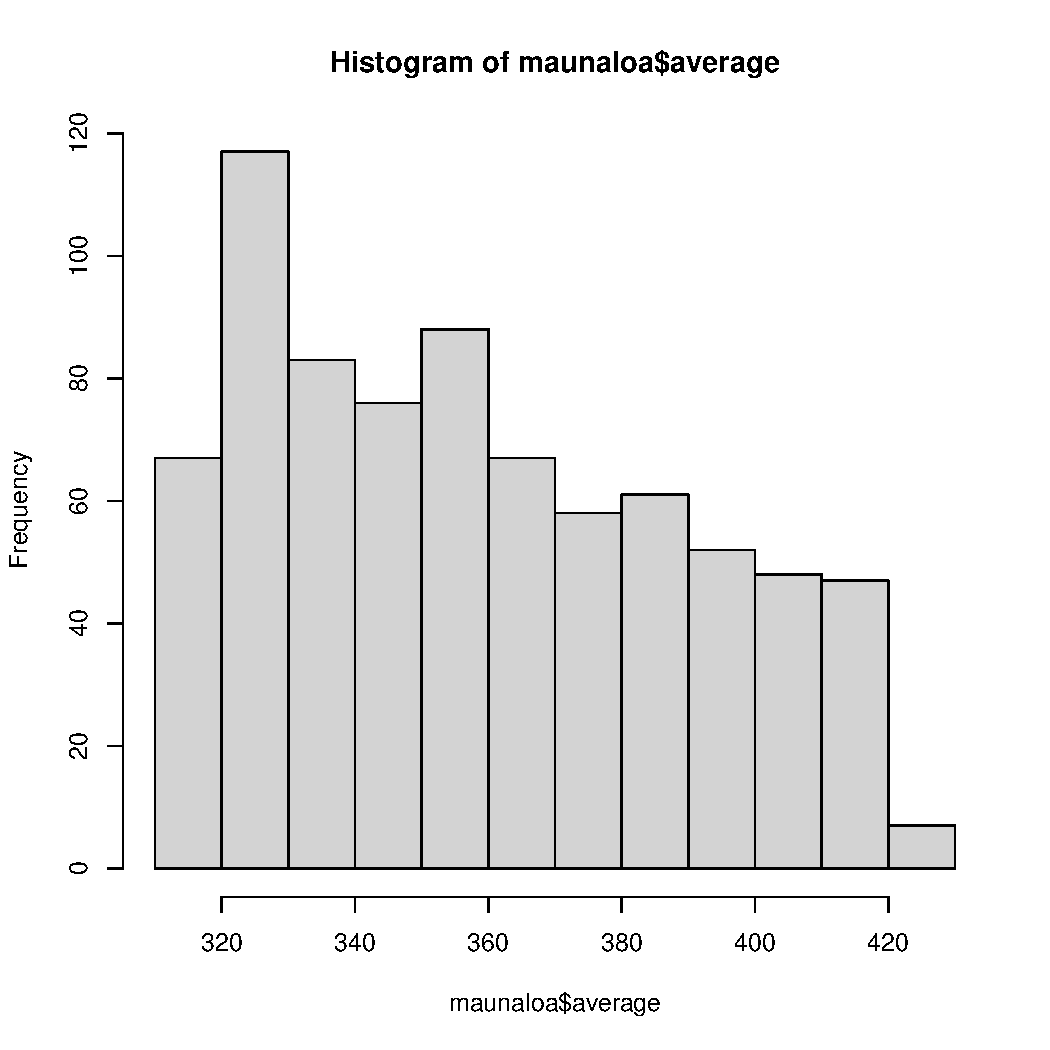
\includegraphics[width=\maxwidth]{figure/unnamed-chunk-44-1} 
\end{knitrout}

The one you have made probably does not look that pretty, but with some more advanced coding, this is what it might look like. 

% Additional LaTeX code to add caption to figure
\begin{marginfigure}[3cm]
\caption{Histogram of carbon dioxide concentrations at Mauna Loa, Hawaii.}
\label{fig:histogram}
\begin{center}
% \setkeys{Gin}{width=0.75\textwidth} % LaTeX code to read the graphic file in at 75% of its original size

% R code chunk that produces a graphic
\begin{knitrout}
\definecolor{shadecolor}{rgb}{0.969, 0.969, 0.969}\color{fgcolor}
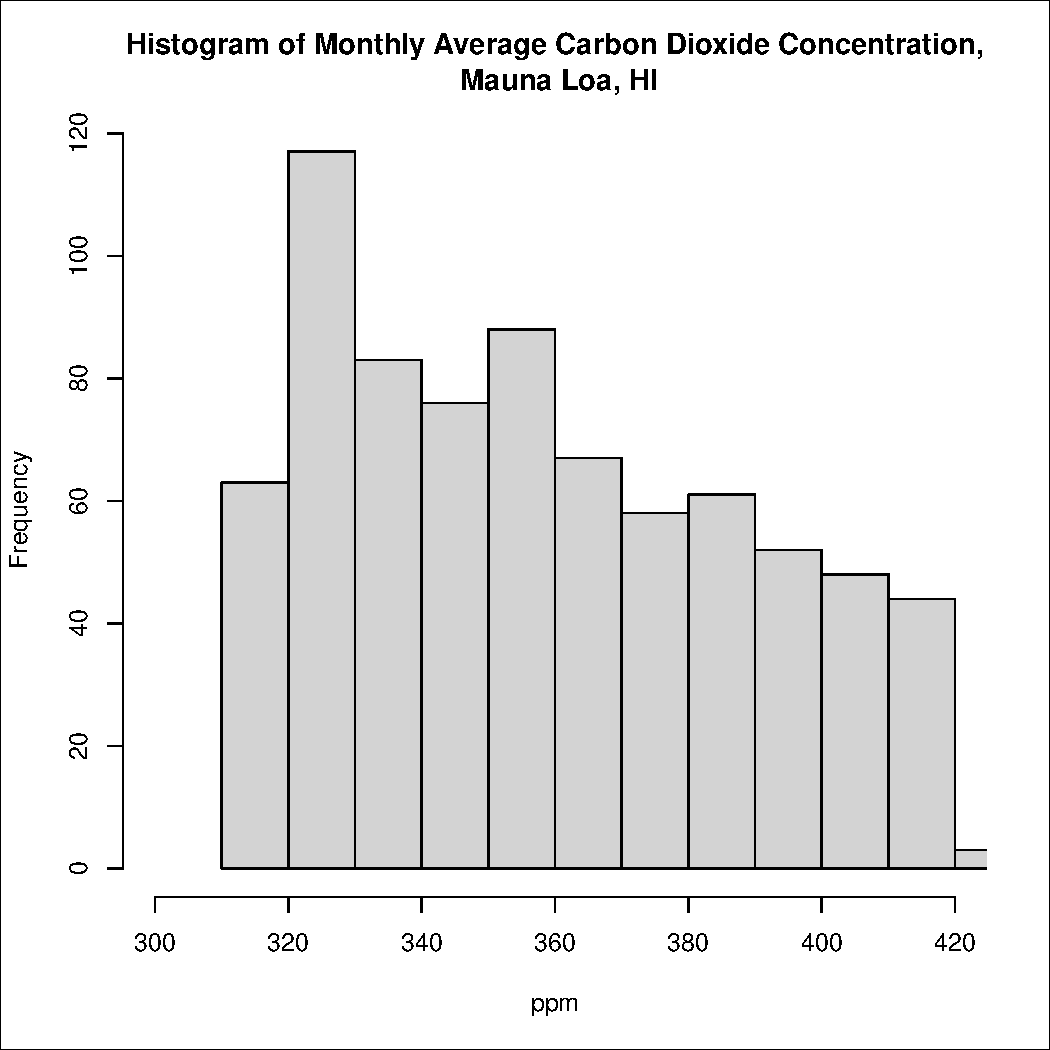
\includegraphics[width=\maxwidth]{figure/unnamed-chunk-45-1} 
\end{knitrout}
\end{center}
\end{marginfigure}

We might also want to learn about the range of measures:

\begin{knitrout}
\definecolor{shadecolor}{rgb}{0.969, 0.969, 0.969}\color{fgcolor}\begin{kframe}
\begin{alltt}
\hlkwd{min}\hlstd{(maunaloa}\hlopt{$}\hlstd{average)}
\hlkwd{max}\hlstd{(maunaloa}\hlopt{$}\hlstd{average)}
\end{alltt}
\end{kframe}
\end{knitrout}

Why do we get errors?  Let's try ignoring missing data:

\begin{knitrout}
\definecolor{shadecolor}{rgb}{0.969, 0.969, 0.969}\color{fgcolor}\begin{kframe}
\begin{alltt}
\hlkwd{min}\hlstd{(maunaloa}\hlopt{$}\hlstd{average,} \hlkwc{na.rm}\hlstd{=T)}
\end{alltt}
\begin{verbatim}
## [1] 313.33
\end{verbatim}
\begin{alltt}
\hlkwd{max}\hlstd{(maunaloa}\hlopt{$}\hlstd{average,} \hlkwc{na.rm}\hlstd{=T)}
\end{alltt}
\begin{verbatim}
## [1] 420.99
\end{verbatim}
\end{kframe}
\end{knitrout}

\noindent These are now a biased measures, just like the mean, median, and standard deviations we calculated before. Can you figure out why?

Congratulations, you have made it through the next step in R!  You now know how to do an exploratory analysis and even generate a basic histogram to view the distribution of a data set. Next, we use a standard statistical technique to determine the slope of the line and weather the line is statistically significant.

\bigskip
\noindent \textbf{\#8 Developing summary statistics is a useful project. What have you learned about these data so far? }

\section{Linear Models in R}

The use of the linear model is the cornerstone of statistics. So ubiquitous it is rarely explained coherently.\sidenote{Outcome: Build and test a linear model.} The linear model can be summarized at the equation for a line, but with the addition of error. You are probably familiar with the equation for a line where, 

\begin{equation}
y = m * x + b
\end{equation}

This equation defines a line, where $m$ is the slope, $b$ is the y-intercept, and the x and y are coordinates. The linear model is based on this form and is usually written as  

\begin{equation}
y \sim \alpha + \beta * x + \epsilon
\end{equation}

The order is usually changed, where the intercept is first, followed by the slope and x variable and the addition of error or noise. The error is usually symbolized as $\epsilon$. In general, in a statistical model, Greek letters are used and instead of an equals sign, we use a tilde, meaning that that left side of the equation is a function of the right side. Luckily, this is the approximate form that R expects, so if you understand this, you will have a pretty good idea of how to code a linear model in R. 

The function to build a linear model is \texttt{lm()}. This function is extremely powerful and can be easily implemented, but this is a good time to see what the help menus look like in R. 

\begin{knitrout}
\definecolor{shadecolor}{rgb}{0.969, 0.969, 0.969}\color{fgcolor}\begin{kframe}
\begin{alltt}
\hlkwd{help}\hlstd{(lm)}
\end{alltt}
\end{kframe}
\end{knitrout}

I am not showing it here, but you should see a long complex looking help page window pop up. All help files in R are structured the same way, so in spite of the uninterpretable text, written by and for computer programmers, the structure will become familiar. Beginning with the description, the help screen describes the function, how to use it, and give some examples. Admittedly, I rarely understand much of the text, but I find the examples to be very useful! In fact, I suggest you paste the example into R and see what happens, I find this one of the best ways to learn R. Use an example that I know works, then change it to make it do what I want it to do.

Using the linear model, we can analyze several types of data, when the response variable is continuous. If the have a predictor variable that is categorical, then we often analyze the data using the method known as analysis of variance or ANOVA. If the predictor variable is continuous, then we often analyze data using a regression analysis. 

Returning the the snow melt data, we will determine if there is a treatment affect on flowering dates due to the treatments (heated, control, and procedure control) First, we create a linear model. Because we want to do an analysis of variance, we use the \texttt{aov()} function, which create an object that can easily be interpreted as an ANOVA table. We could also use the \texttt{lm()} function, which you might try as well to see the difference. 

\begin{knitrout}
\definecolor{shadecolor}{rgb}{0.969, 0.969, 0.969}\color{fgcolor}\begin{kframe}
\begin{alltt}
\hlstd{Flowering.aov} \hlkwb{<-} \hlkwd{aov}\hlstd{(Flowering_date} \hlopt{~} \hlstd{Treatment,} \hlkwc{data}\hlstd{=Flowering)}
\end{alltt}
\end{kframe}
\end{knitrout}

By creating the linear model, the \texttt{aov()} function create an object that can then be interrogated to see the results.\sidenote[][-.5cm]{There is a tilde ($\sim$) between Flowering\_date and Treatment, which can be read as ``a function of''.} Using a \texttt{summary()} function, R returns

\begin{knitrout}
\definecolor{shadecolor}{rgb}{0.969, 0.969, 0.969}\color{fgcolor}\begin{kframe}
\begin{alltt}
\hlkwd{summary}\hlstd{(Flowering.aov)}
\end{alltt}
\begin{verbatim}
##             Df Sum Sq Mean Sq F value Pr(>F)  
## Treatment    2  170.8   85.40   4.022  0.046 *
## Residuals   12  254.8   21.23                 
## ---
## Signif. codes:  
## 0 '***' 0.001 '**' 0.01 '*' 0.05 '.' 0.1 ' ' 1
\end{verbatim}
\end{kframe}
\end{knitrout}

The output shows the sum of squares, the mean sum of squares, the F value and the p-value. We'll spend some time reviewing these so you can interpret these data correctly each time.

Notice the syntax for the linear model. It is quite abbreviated. There are not coefficients and no error term defined. Why?  This form of model specification was proposed by statisticians in the late 1960s and it has become standard practice in computer coding. It does require some translation between a statistics book and the computer code. This is why I recommend stats books that are written for R.  

Okay, let's see if we can do this for our Mauna Loa data. Let's test if there is a significant change of carbon dioxide concentrations with time. Since both the predictor and response variables are continuous data, this analysis will be a linear regression, but the form and function of the linear model are exactly the same. The linear model would look something like this

\begin{equation}
CO_2 \sim \alpha + \beta * time + \epsilon
\end{equation}

Translating this in R will take some additional tricks besides just getting the code figured out. First, we need to identify the predictor variable in the data frame. There are three variables associated with time: year, month, and decimal.date. Because these data are in a time series, they are serially correlated, meaning that the June sample will be more like the July sample than the August sample. In addition, the June 2010 sample will be similar to the June 2009 sample. These correlation violate the assumption of independence, but for today, we will ignore this violation and just create a linear model in bliss. So, let's use year as the predictor variable and assume there might be some error because each month have slightly different concentrations. For the response variable, we will use the monthly averages, "average". Remember there are some missing data, it will be interesting to note how R deals with that.

First, let's create a plot of data using \texttt{plot()}, whose format is \texttt{plot(x, y)} or \texttt{plot(y ~ x)}. We will use the later for now, 

\begin{knitrout}
\definecolor{shadecolor}{rgb}{0.969, 0.969, 0.969}\color{fgcolor}\begin{kframe}
\begin{alltt}
\hlkwd{plot}\hlstd{(average} \hlopt{~} \hlstd{year,} \hlkwc{data}\hlstd{=maunaloa)}
\end{alltt}
\end{kframe}
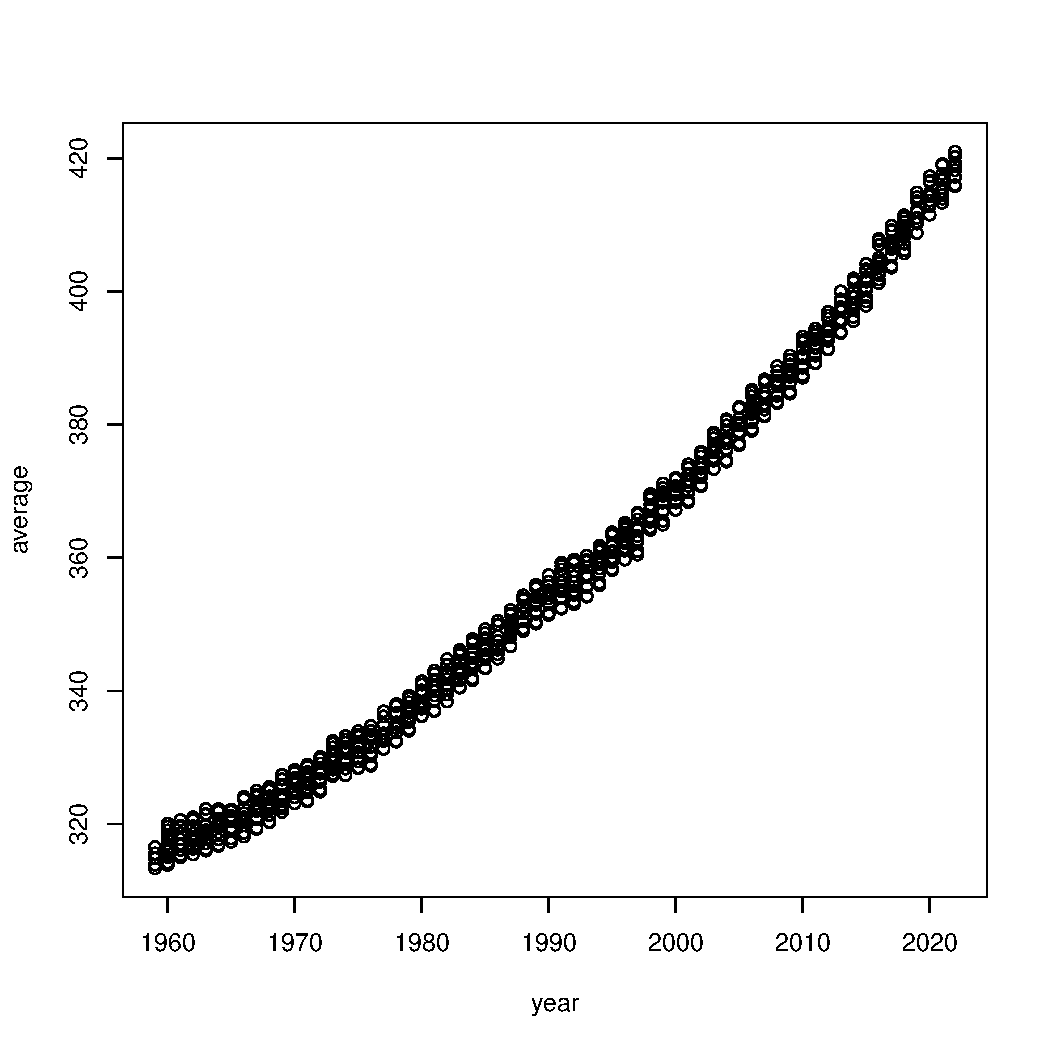
\includegraphics[width=\maxwidth]{figure/unnamed-chunk-51-1} 
\end{knitrout}


\begin{figure}
\label{fig:maunaloa}
\caption{Carbon dioxide concentrations sampled for each month at Mauna Loa, Hawaii.}
\begin{knitrout}
\definecolor{shadecolor}{rgb}{0.969, 0.969, 0.969}\color{fgcolor}
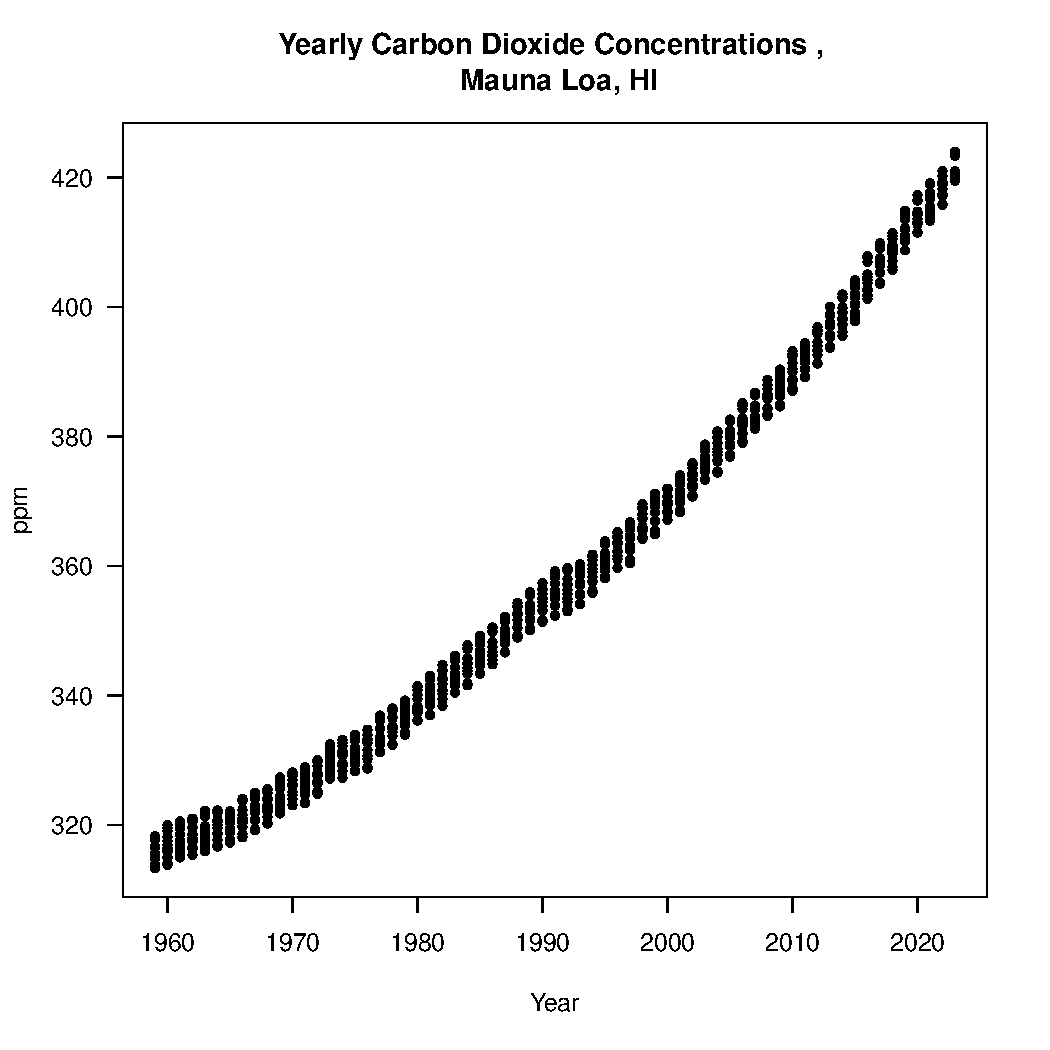
\includegraphics[width=\maxwidth]{figure/unnamed-chunk-52-1} 
\end{knitrout}
\end{figure}


Finally, there is one important difference between the linear model that we used in the \texttt{aov()} function. This time we use the \texttt{lm()} function that arrange the results more in-line with a regression model.
This syntax is still pretty straight forward,  

\begin{knitrout}
\definecolor{shadecolor}{rgb}{0.969, 0.969, 0.969}\color{fgcolor}\begin{kframe}
\begin{alltt}
\hlkwd{lm}\hlstd{(average} \hlopt{~} \hlstd{year,} \hlkwc{data}\hlstd{=maunaloa)}
\end{alltt}
\begin{verbatim}
## 
## Call:
## lm(formula = average ~ year, data = maunaloa)
## 
## Coefficients:
## (Intercept)         year  
##   -2889.767        1.632
\end{verbatim}
\end{kframe}
\end{knitrout}

From this model, we learn that the change in $CO_2$ is 1.63 ppm $year^{-1}$.\sidenote{When I first made this handout the rate of increase was 1.441. Why do you think this rate has changed?} Figure~\ref{fig:maunaloa} shows the increasing concentrations, but also the seasonal variation. Statisticians have more advanced methods to analyze these data then what we have done, but for our purposes the implications are the same.  Greenhouse gas emissions are increasing and the estimated rates suggest an increasing rate.

% Additional LaTeX code to add caption to figure
\begin{figure*}
\label{fig:maunaloa}
\caption{Carbon dioxide concentrations at Mauna Loa, Hawaii. NOTE: This graphic is different from what you made. See if you can make yours look more like this, using these functions: \texttt{coef()} and \texttt{abline()}.}
\begin{knitrout}
\definecolor{shadecolor}{rgb}{0.969, 0.969, 0.969}\color{fgcolor}
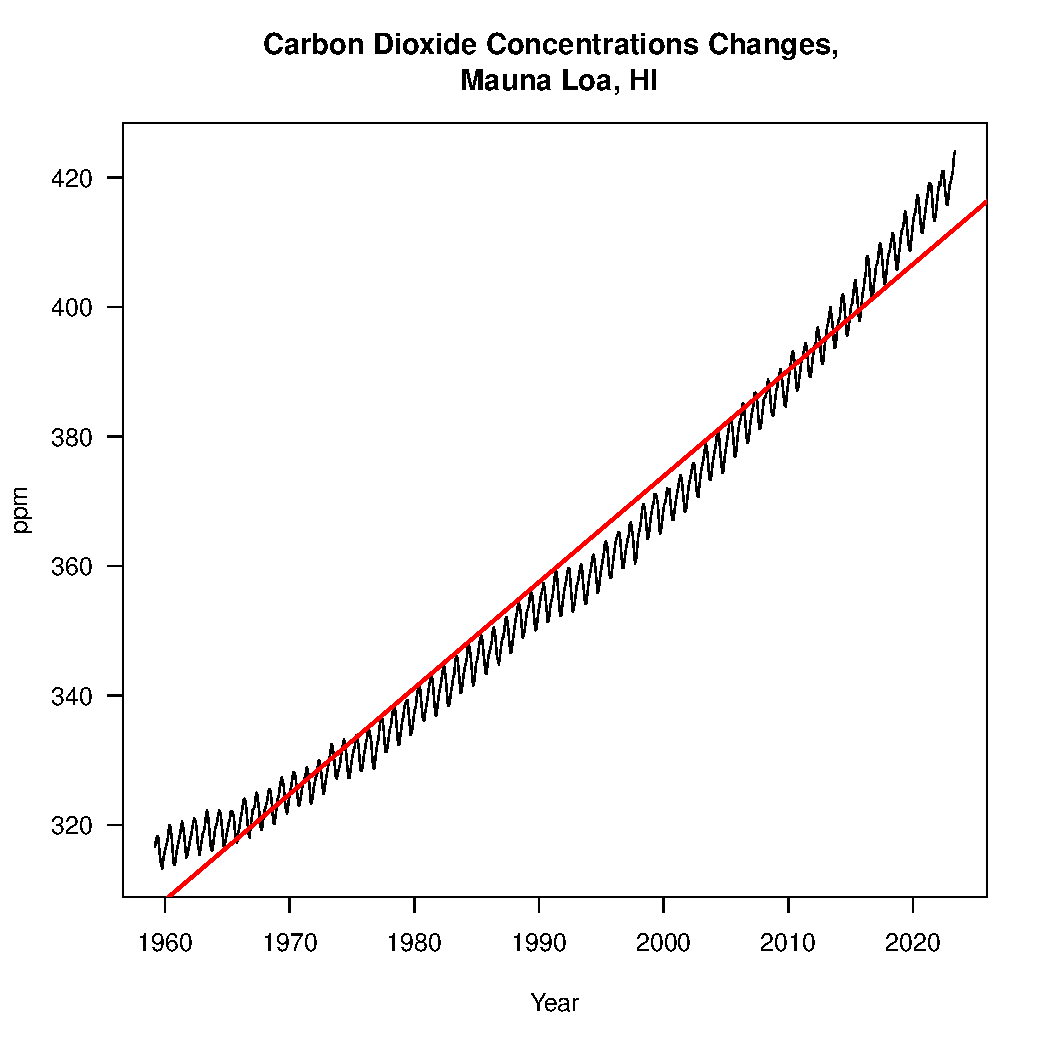
\includegraphics[width=\maxwidth]{figure/unnamed-chunk-54-1} 
\end{knitrout}
\end{figure*}

Now let's ask if this value is significant, by putting the linear model into a ANOVA-like table. There are a number of functions that do this and we have seen the \texttt{anova()} function above. For linear regression, however, the \texttt{summary()} function gives a more complete output.

\begin{knitrout}
\definecolor{shadecolor}{rgb}{0.969, 0.969, 0.969}\color{fgcolor}\begin{kframe}
\begin{alltt}
\hlkwd{summary}\hlstd{(}\hlkwd{lm}\hlstd{(average} \hlopt{~} \hlstd{year,} \hlkwc{data}\hlstd{=maunaloa))}
\end{alltt}
\begin{verbatim}
## 
## Call:
## lm(formula = average ~ year, data = maunaloa)
## 
## Residuals:
##     Min      1Q  Median      3Q     Max 
## -8.3420 -3.3146 -0.8853  2.6741 11.6317 
## 
## Coefficients:
##               Estimate Std. Error t value Pr(>|t|)    
## (Intercept) -2.890e+03  1.730e+01  -167.0   <2e-16 ***
## year         1.632e+00  8.693e-03   187.7   <2e-16 ***
## ---
## Signif. codes:  
## 0 '***' 0.001 '**' 0.01 '*' 0.05 '.' 0.1 ' ' 1
## 
## Residual standard error: 4.365 on 756 degrees of freedom
## Multiple R-squared:  0.979,	Adjusted R-squared:  0.979 
## F-statistic: 3.523e+04 on 1 and 756 DF,  p-value: < 2.2e-16
\end{verbatim}
\end{kframe}
\end{knitrout}

Here we find the that the slope and intercept are highly significant, we have some information on the residuals, and $R^2$ estimates, etc.

\bigskip
\noindent  \textbf{\#9 The Muana Loa data are the most recent data available. What are some patterns that you might glean from the graphics you made so far? }

\section{Model Diagnostics}

With every statistical test done, researchers validate their model in some way or anther. Often this entails the use of diagnostics, a standardize battery of procedures to check to see if the data are following the assumptions. 

In R four plots are created by default.  To see them all at the same time, we need to change the graphical parameters so the graphics window expects four panels, in this case a 2 rows and two columns. 

\begin{knitrout}
\definecolor{shadecolor}{rgb}{0.969, 0.969, 0.969}\color{fgcolor}\begin{kframe}
\begin{alltt}
\hlkwd{par}\hlstd{(}\hlkwc{mfrow}\hlstd{=}\hlkwd{c}\hlstd{(}\hlnum{2}\hlstd{,}\hlnum{2}\hlstd{))}
\end{alltt}
\end{kframe}
\end{knitrout}

Try not to get bogged down in the code at this point. But it is a useful thing to remember.

% Additional LaTeX code to add caption to figure
\begin{figure}
\label{fig:diagnostics}
\caption{Default diagnostic plots for a linear model in R.}
%\setkeys{Gin}{width=0.75\textwidth} % LaTeX code to read the graphic file in at 75% of its original size
% R code chunk that produces a graphic
\begin{knitrout}
\definecolor{shadecolor}{rgb}{0.969, 0.969, 0.969}\color{fgcolor}\begin{kframe}
\begin{alltt}
\hlkwd{par}\hlstd{(}\hlkwc{mfrow}\hlstd{=}\hlkwd{c}\hlstd{(}\hlnum{2}\hlstd{,}\hlnum{2}\hlstd{))}
\hlkwd{plot}\hlstd{(}\hlkwd{lm}\hlstd{(average} \hlopt{~} \hlstd{year,} \hlkwc{data}\hlstd{=maunaloa))}
\end{alltt}
\end{kframe}
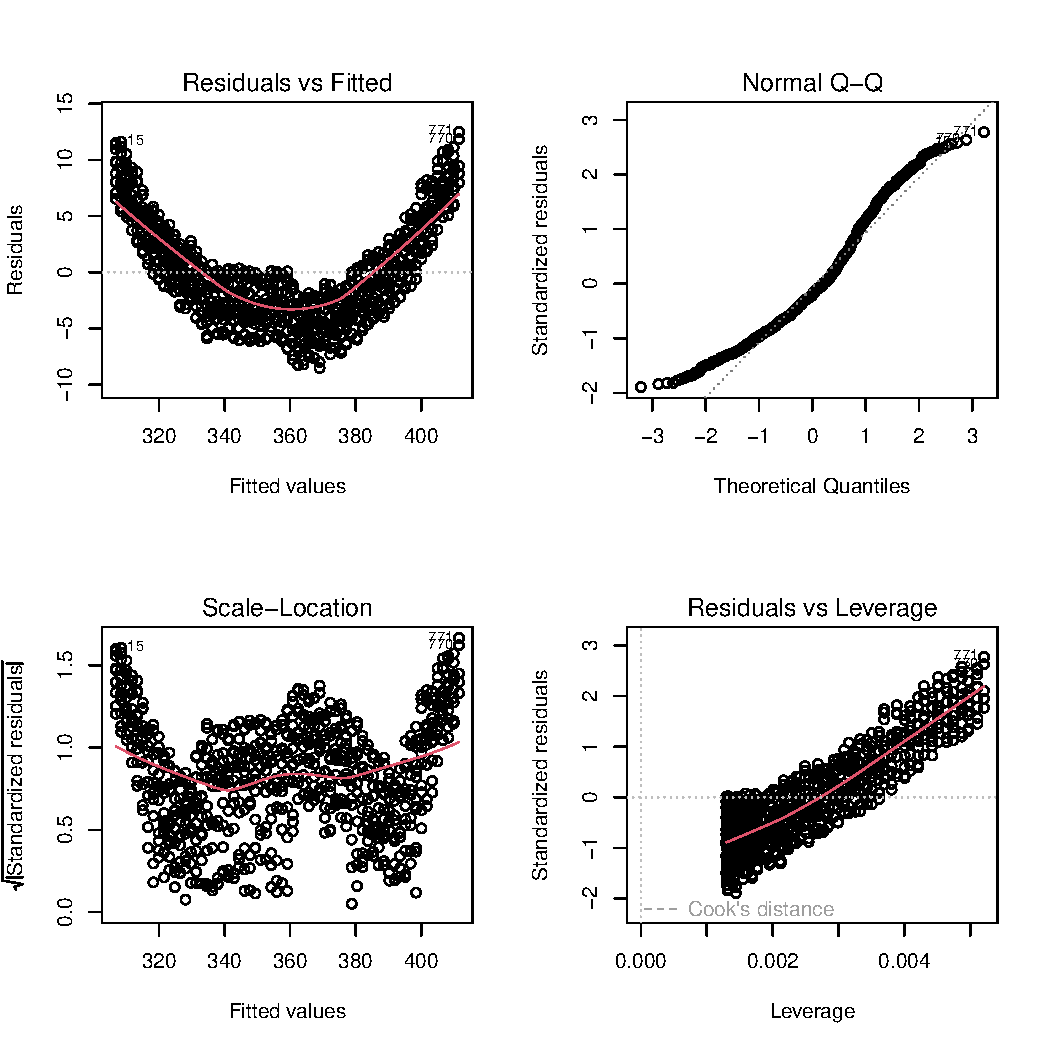
\includegraphics[width=\maxwidth]{figure/unnamed-chunk-57-1} 
\begin{kframe}\begin{alltt}
\hlkwd{par}\hlstd{(}\hlkwc{mfrow}\hlstd{=}\hlkwd{c}\hlstd{(}\hlnum{1}\hlstd{,}\hlnum{1}\hlstd{))}
\end{alltt}
\end{kframe}
\end{knitrout}
\end{figure}

To determine the validity of linear model assumptions (\eg normality or heterogeneity of variance), you have probably used statistical tests; in contrast statisticians almost exclusively look at diagnostic plots. Why?  When assumptions are violated the tests to determine violations do not perform well. So, let's see how to look at these assumptions graphically with these diagnostic plots. Linear models should have diagnostic plots that do not have any obvious structure or pattern. In this case, Figure~\ref{fig:diagnostics} should show a great deal remaining structure in the residuals. Although for today, we are not going to try to interpret these figures, but you should notice there is a ton of unaccounted structure, \ie variance, in the model. This is due, in part, to a violation of independence; these data are serially correlated and the model does not account for that and is inappropriate because of this. It also appears that a straight-line model does not fit well and a curvilinear should be investigated. 

A properly specified model is shown in Figure~\ref{fig:co2_data_mlo}. In this case, the trend line has been developing using a time series analysis, which is beyond the scope of this course. Nevertheless, you want to keep this in mind during the semester because we will see a fair amount of data that looks like this.

\begin{figure}
	\includegraphics{co2_data_mlo.pdf}
	\caption{Properly Specified Model (red trend line) for Carbon Dioxide Changes}
	\label{fig:co2_data_mlo}
\end{figure}

\bigskip
\noindent \textbf{\#10 What is the difference between a linear model and a properly specified model of carbon dioxide changes?  What kinds of resources might you need to determine which is the best model?}

\section{Creating a Tufte Figure}

Creating a figure for professional manuscripts or reports requires careful attention. To develop a good figure it helps to have some guiding principles. For many scientists, they rely on the writings and advice of Edward Tufte\sidenote{Outcome: Create a publication quality graphics using the principles of \citet{Tufte:1983, Tufte:1997}}. Tufte argues that all the ink used in making a figure must communicate information; if there is ink that does not, then it should be removed from the figure. The goal of every figure should be to maximize the information to ink ratio. Granted, I don't know how one could measure this ratio, but the point is well taken. Luckily, R is a great place to begin, because it is both flexible and does not generate a great deal of extra junk that can get in the way. The drawback is that there are many options; and sometimes a complex syntax is required to get the figures to cooperate. However, I think this handout will get you pretty far.  

Let's start by making a scatter plot. Returning to our Michaelis-Menten Equation, let's graph the results of nutrient uptake rates of various phytoplankton species. 

\begin{margintable}
	\caption{Phytoplankton Parameters from \citep{REF}.}
		\begin{tabular}{lcc}
		\toprule
Species &\ $V_{max}$\ & $K_s$ \\
\midrule
Cyanobacteria & 0.3 & 1.5 \\
Diatoms 			& 0.2 & 2.5 \\
Green Algae   & 0.1 & 1.0 \\	
\bottomrule
		\end{tabular}
	\label{tab:PhytoplanktonParameters}
\end{margintable}

Based on Table~\ref{tab:PhytoplanktonParameters}, let's crate a scatter plot for Cyanobacteria. The command to create a plot is appropriately named: \texttt{plot()}. The function expects x-axis variables and then y-axis variables in order. However, to be explicit, thus the order is less critical, we'll define them in the function.

First, let's make sure create the objects to be used in the plot, \ie the x axis (substrate concentration, S) and each of the response variables, the V for each phytoplankton (Macro

\begin{knitrout}
\definecolor{shadecolor}{rgb}{0.969, 0.969, 0.969}\color{fgcolor}\begin{kframe}
\begin{alltt}
\hlstd{S} \hlkwb{<-} \hlkwd{seq}\hlstd{(}\hlnum{0}\hlstd{,}\hlnum{2}\hlstd{,} \hlnum{0.002}\hlstd{)}
\hlstd{V_cyano}   \hlkwb{<-} \hlkwd{mm}\hlstd{(}\hlnum{0.3}\hlstd{,} \hlnum{1.5}\hlstd{, S)}
\hlstd{V_diatoms} \hlkwb{<-} \hlkwd{mm}\hlstd{(}\hlnum{0.2}\hlstd{,} \hlnum{2.5}\hlstd{, S)}
\hlstd{V_green}   \hlkwb{<-} \hlkwd{mm}\hlstd{(}\hlnum{0.1}\hlstd{,} \hlnum{0.004}\hlstd{, S)}
\end{alltt}
\end{kframe}
\end{knitrout}

Check to make sure the cyano vector (which are the Vs, but we'll call them cyano, since we'll eventually have three different Vs). So, now we want to graph these, with the plot function.

\begin{knitrout}
\definecolor{shadecolor}{rgb}{0.969, 0.969, 0.969}\color{fgcolor}\begin{kframe}
\begin{alltt}
\hlkwd{plot}\hlstd{(}\hlkwc{x}\hlstd{=S,} \hlkwc{y}\hlstd{=V_cyano)}
\end{alltt}
\end{kframe}
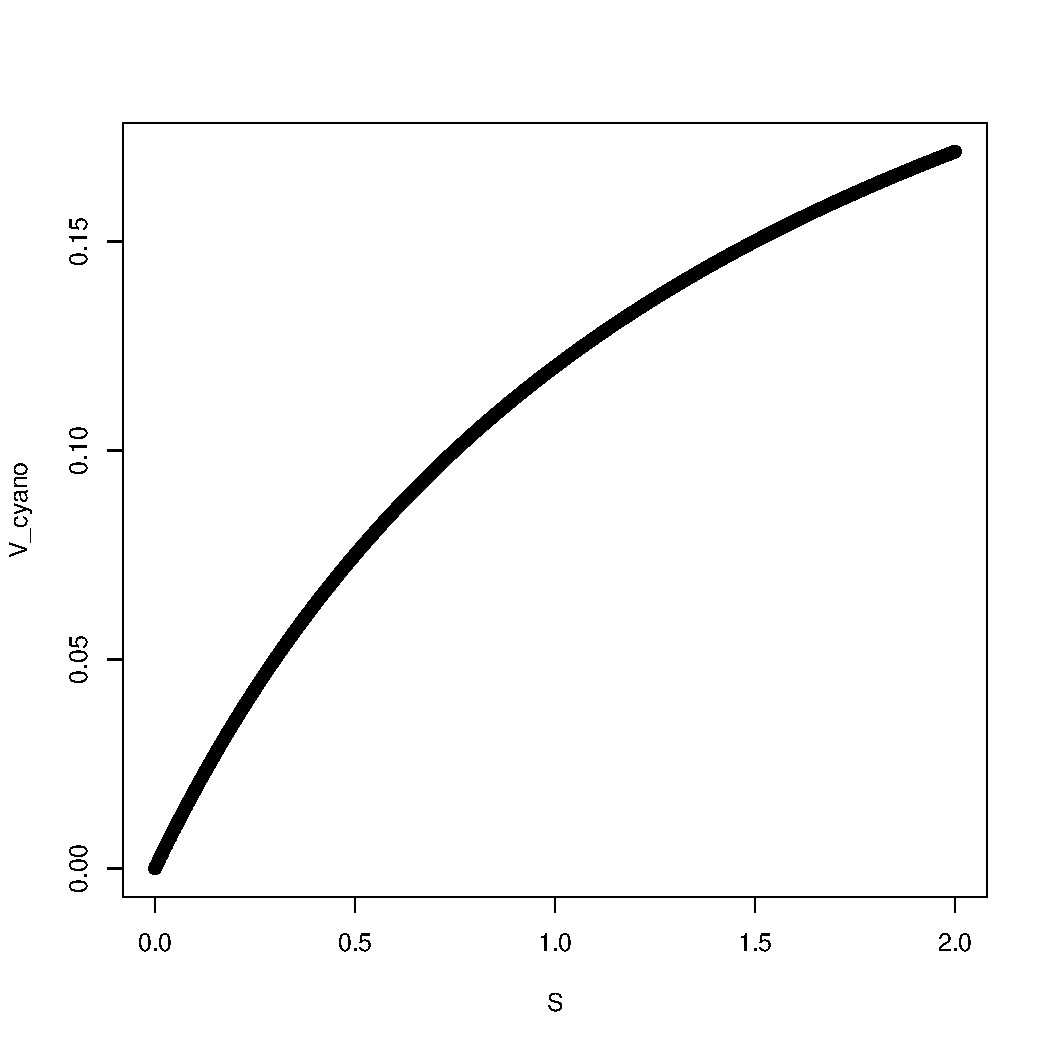
\includegraphics[width=\maxwidth]{figure/unnamed-chunk-59-1} 
\end{knitrout}

That was easy. However, we still have not created of Tufte figure. First let's improve the figure with better clarity and appropriate types of design. Since the substrate concentrations are more or less continuous and we can assume that points between existing points will lie on a line, lets covert the figure to a line graph, with \texttt{type="l"}.\sidenote{NOTE: This is the letter 'l' for line, not the number 1!} And since we might be able to make a few changes as one.  So, let's add labels to the x and y axes, with \texttt{xlab=" "} and \texttt{ylab=" "} and putting something in between the quotations marks.  Let's try what we have so far,

\begin{knitrout}
\definecolor{shadecolor}{rgb}{0.969, 0.969, 0.969}\color{fgcolor}\begin{kframe}
\begin{alltt}
\hlkwd{plot}\hlstd{(}\hlkwc{x}\hlstd{=S,} \hlkwc{y}\hlstd{=V_cyano,} \hlkwc{xlab}\hlstd{=}\hlstr{"Substrate Concentration"}\hlstd{,} \hlkwc{ylab}\hlstd{=}\hlstr{"Uptake Rate"}\hlstd{,} \hlkwc{type}\hlstd{=}\hlstr{"l"}\hlstd{)}
\end{alltt}
\end{kframe}
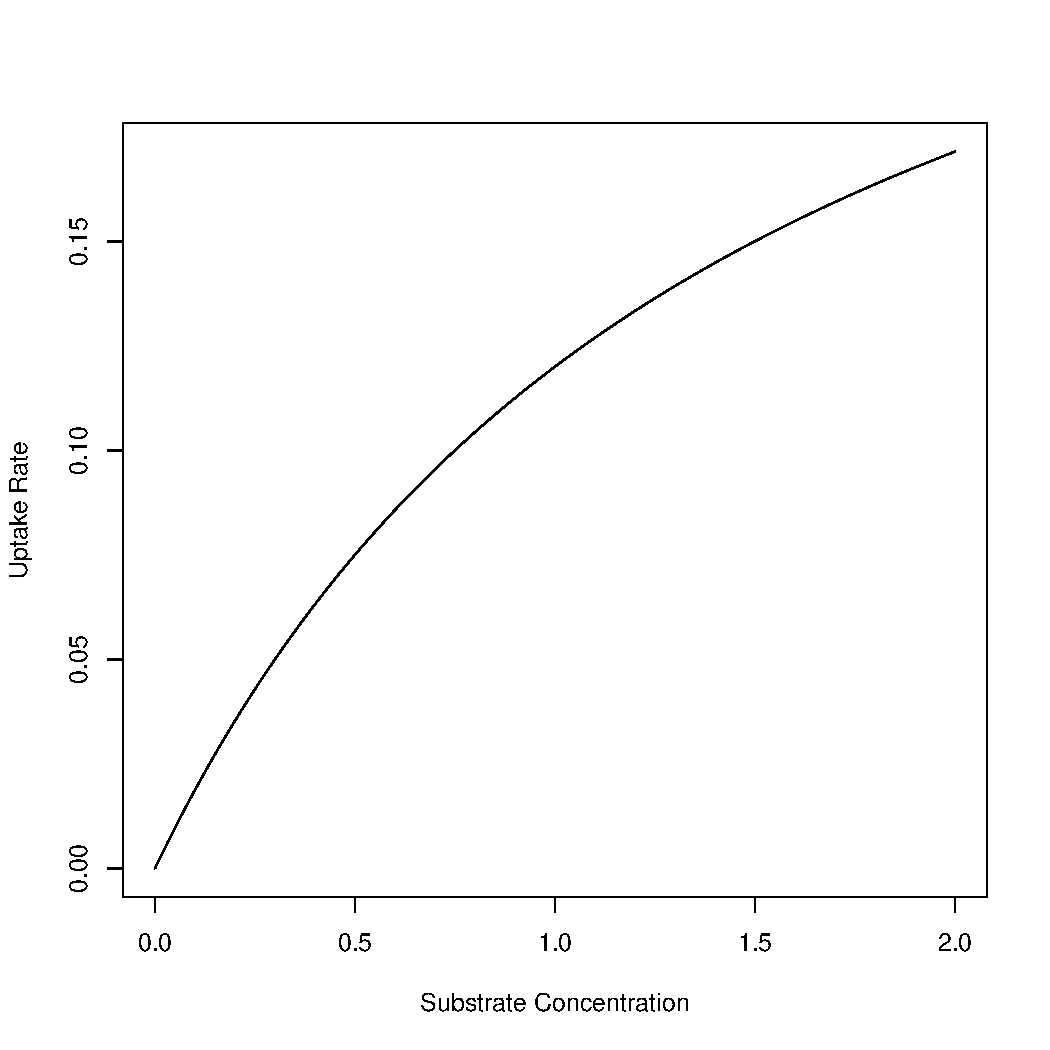
\includegraphics[width=\maxwidth]{figure/unnamed-chunk-60-1} 
\end{knitrout}

Good, Okay, we have created a figure that has much of the information needed. Now we need to figure out if the figure is going to have a title. In Excel, we often click on the main title and stick something in there out of habit. However, habit does not serve us as we create figures in science. Keep in mind that Excel defaults have been created for business applications, not science, so most of the defaults are something you need to be critical of. Compare the figures in Excel to what you see in scientific papers!  Okay, let's get back on track. So, you can add a title, by adding \texttt{main=""}, however, I am going to recommend that you don't. Instead, we use the caption to describe the figure and what the reader should be getting out of it.  So we'll work on that in a few minutes too. But first, let's get rid of stuff that is not helping. For example, what does the frame around the figure provide? Perhaps nothing.  We need a single x-axis and a single y-axis.  We don't need the lines on the right and top, you can use \texttt{frame.plot=F} to remove the frame from the plot, which I did below.\sidenote{Note, the \# symbol denotes the beginning of a comment in R. R will ignore these comments and are present to document what various codes are attempting to accomplish.}  Also, it's a good idea to thicken the line in the graph with a line width command (\texttt{lwd}), which has a default of 1, let's try 3. When you put this figure in a paper, lab report or presentation, you'll find that these tricks can increase the clarity. Science is complicated, so anything we can to to clarify stuff with better figures, the better.





% R code chunk that produces a graphic
\begin{knitrout}
\definecolor{shadecolor}{rgb}{0.969, 0.969, 0.969}\color{fgcolor}\begin{kframe}
\begin{alltt}
\hlkwd{par}\hlstd{(}\hlkwc{las}\hlstd{=}\hlnum{1}\hlstd{,} \hlkwc{cex}\hlstd{=}\hlnum{1.5}\hlstd{,} \hlkwc{mar}\hlstd{=}\hlkwd{c}\hlstd{(}\hlnum{4}\hlstd{,}\hlnum{4.5}\hlstd{,}\hlnum{0}\hlstd{,}\hlnum{1}\hlstd{))}
\hlcom{# Example from Foin, 1994}
\hlkwd{plot}\hlstd{(S,V_cyano,} \hlkwc{xlab}\hlstd{=}\hlkwd{expression}\hlstd{(}\hlkwd{paste}\hlstd{(}\hlstr{"Available Nitrogen ("}\hlstd{, mg} \hlopt{~~} \hlstd{L}\hlopt{^-}\hlnum{1}\hlstd{,} \hlstr{")"}\hlstd{)),}
  \hlkwc{ylab}\hlstd{=}\hlkwd{expression}\hlstd{(}\hlkwd{paste}\hlstd{(}\hlstr{"Nitrogen Uptake Rate ( "}\hlstd{, mg} \hlopt{~~} \hlstd{g}\hlopt{^-}\hlnum{1} \hlopt{~~} \hlstd{h}\hlopt{^-}\hlnum{1}\hlstd{,} \hlstr{")"}\hlstd{)),}
        \hlkwc{lty}\hlstd{=}\hlnum{1}\hlstd{,} \hlkwc{col}\hlstd{=}\hlstr{"seagreen"}\hlstd{,} \hlkwc{lwd}\hlstd{=}\hlnum{3}\hlstd{,} \hlkwc{ylim}\hlstd{=}\hlkwd{c}\hlstd{(}\hlnum{0}\hlstd{,}\hlnum{0.2}\hlstd{),} \hlkwc{xlim}\hlstd{=}\hlkwd{c}\hlstd{(}\hlnum{0}\hlstd{,}\hlnum{2}\hlstd{),} \hlkwc{type}\hlstd{=}\hlstr{"l"}\hlstd{,} \hlkwc{frame.plot}\hlstd{=F)}

\hlcom{# Add second and third line}
\hlkwd{lines}\hlstd{(S,V_diatoms,} \hlkwc{col}\hlstd{=}\hlstr{"blue"}\hlstd{,} \hlkwc{lwd}\hlstd{=}\hlnum{3}\hlstd{,} \hlkwc{lty}\hlstd{=}\hlnum{2.6}\hlstd{)}
\hlkwd{lines}\hlstd{(S,V_green,} \hlkwc{col}\hlstd{=}\hlstr{"purple"}\hlstd{,} \hlkwc{lwd}\hlstd{=}\hlnum{3}\hlstd{,} \hlkwc{lty}\hlstd{=}\hlnum{3}\hlstd{)}

\hlcom{# Add legend(x, y, plus some text, symbols, colors, line type, line width, box, and size)}
\hlkwd{legend}\hlstd{(}\hlnum{.8}\hlstd{,} \hlnum{0.05}\hlstd{,} \hlkwd{c}\hlstd{(}\hlstr{"Cyanobacteria"}\hlstd{,} \hlstr{"Diatoms"}\hlstd{,} \hlstr{"Green Algae"}\hlstd{),} \hlkwc{col}\hlstd{=}\hlkwd{c}\hlstd{(}\hlstr{"seagreen"}\hlstd{,} \hlstr{"blue"}\hlstd{,} \hlstr{"purple"}\hlstd{),}
\hlkwc{lty}\hlstd{=}\hlkwd{c}\hlstd{(}\hlnum{1}\hlstd{,}\hlnum{2}\hlstd{,}\hlnum{3}\hlstd{),} \hlkwc{lwd}\hlstd{=}\hlnum{3}\hlstd{,} \hlkwc{bty}\hlstd{=}\hlstr{"n"}\hlstd{,} \hlkwc{cex}\hlstd{=}\hlnum{1.1}\hlstd{)}
\end{alltt}
\end{kframe}
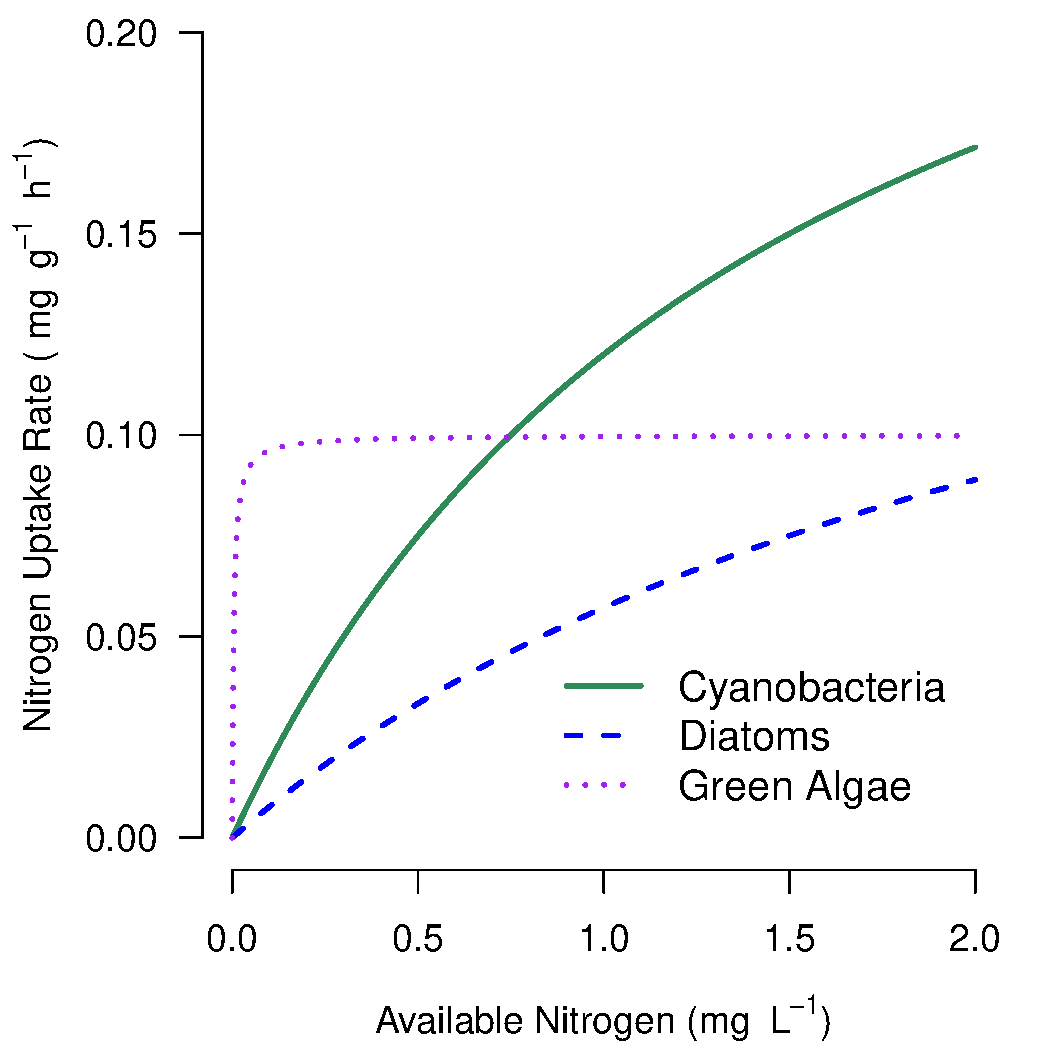
\includegraphics[width=\maxwidth]{figure/a-1} 
\end{knitrout}

Figure~\ref{fig:michaelis} demonstrates a well known relationship between changes in uptake rates based on different enzymatic characteristics. As it turns out these characteristics have do a pretty good job predicting phytoplankton dynamics in lakes based on nutrient concentrations. However, for our purposes, it is important to notice certain characteristics regarding the figure design:

\begin{itemize}
	\item Axes are clearly labeled that include units
	\item The legend is large enough to see and read
	\item The lines can be interpreted in a color and black and white scheme.
\end{itemize}

% Additional LaTeX code to add caption to figure
\begin{figure}
\caption{Substrate and uptake rate of nitrogen comparing various phytoplankton.}
\label{fig:michaelis}
\begin{knitrout}
\definecolor{shadecolor}{rgb}{0.969, 0.969, 0.969}\color{fgcolor}
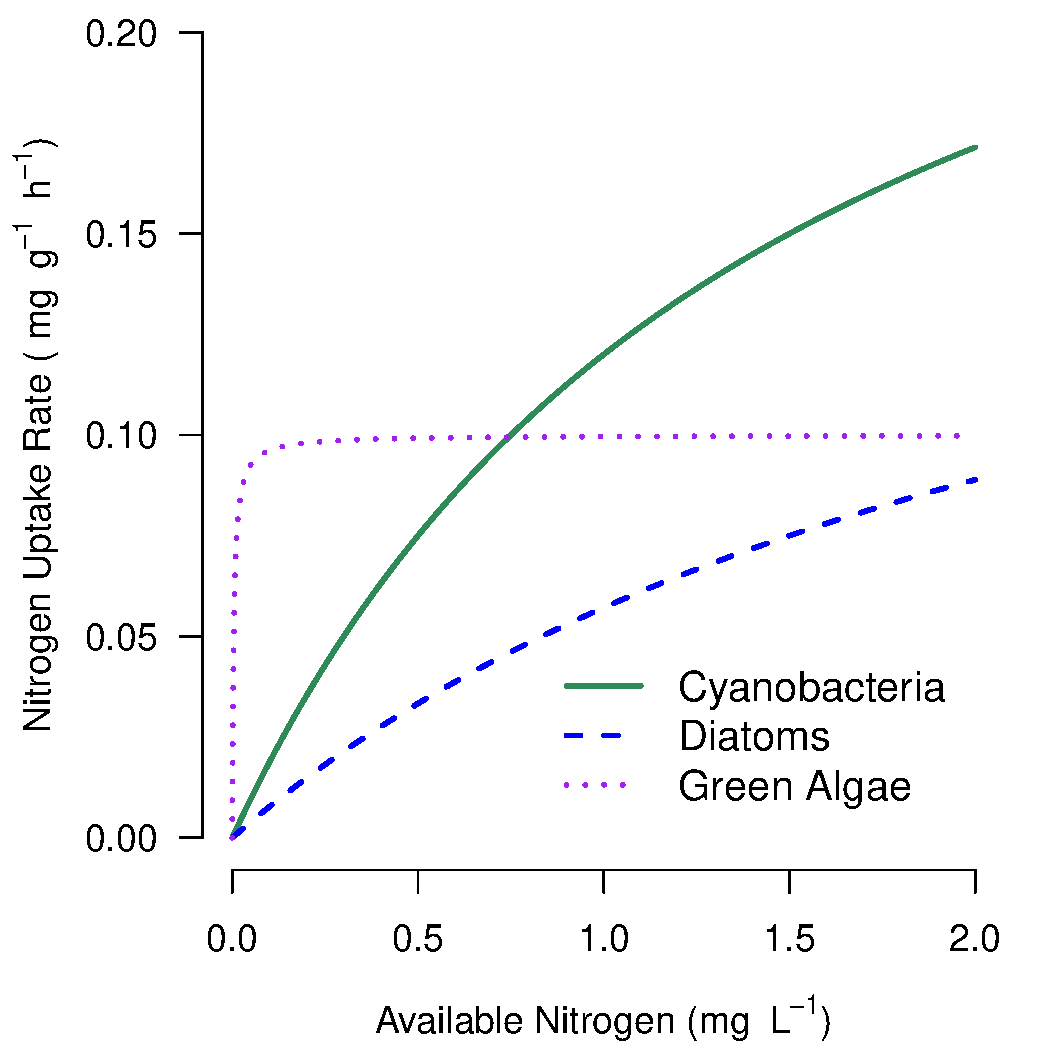
\includegraphics[width=\maxwidth]{figure/unnamed-chunk-63-1} 
\end{knitrout}
\end{figure}


Learning how to do all this, will take some time and takes a fair amount of trial and error. Unfortunately, in contrast to Excel, you can't just click on a particular part of the graph and change it. However, over time, you will get pretty good at copying and modifying code that you have already created so the time you need to create effective graphics will go down dramatically.

\bigskip
\noindent \textbf{\#11 Creating functions allows you to customize and process repetitive data easily (more or less!). List several examples that you could envision using functions in this class. }

\bigskip
\noindent \textbf{\#12 Creating figures is a great way to communicate quantitative data. What would you like to add to make the figures in this handout more clear to you?}

\section{Conclusion}
So, this completes the introduction to R. The program is extremely flexible, but this flexibility comes with a costs. It is easy to get confused between different methods to accomplish stuff. Nevertheless, for a programming environment, the software seems to have provide an opportunity to learn a number of the computing skills needed in across a wide range of potential careers. 

There are several things that I think are worth considering when using R. The software is developing quickly and its use in colleges and universities is expanding dramatically, in part because of the costs. Also, there are a number of tools growing to improve the GUI, for example, RCommander and RExcel packages are improve access to the program dramatically. Finally, R is showing up more and more in job descriptions, and it appears this trend will continue. 
\clearpage

\FloatBarrier 
\begin{fullwidth}
% \renewcommand{\bibfont}{\small}
\bibliography{LosHuertos_Complete_100420}
\bibliographystyle{cbe}
\end{fullwidth}


\newpage\newpage
\begin{fullwidth}
\section{Pre- and Post-Session Evaluation}

\subsection{Pre-Session Assessment}
\begin{enumerate}
	\item Before we begin, please rank your computability with various computer technologies (5= highly comfortable, 0 = completely new) :
	
\begin{table}
		\begin{tabular}{|l|l|} \toprule
Technology					& Rating \\ \midrule
Apple Computer Hardware Setup 										& \\
Apple Software Installation and Use								& \\
PC Computer Hardware Setup												& \\
PC Computer Software Installation and Use					& \\
Using Excel to make calculations									& \\
Using Excel to make graphics											& \\
Using command line software												& \\
Computer Programming to solve equations						& \\
Computer programming to solve repetitive calculations & \\
Use computers to calculate statistics							& \\
		\bottomrule
		\end{tabular}
\end{table}	
	
	\item Rate your confidence with the following outcomes (Task can be independently accomplished with confidence = 5; Task cannot be independently accomplished with confidence = 0).
	
\begin{table}
		\begin{tabular}{|l|l|l|} \toprule
Outcome						& Before & After \\ \midrule
Open and use the R GUI with consistent results 		&& \\
Use math operators to solve simple calculations		&& \\
Create objects																		& &\\
Solve repetitive calculations										&	& \\
Make a function																		&& \\
Get data into the R environment										&& \\
Generate summary statistics												& &\\
Build and test a linear model										&	& \\
Create publication quality graphics								&& \\
		\bottomrule
		\end{tabular}
\end{table}

\subsection{Post-Session Assessment}

Using a word process, address each of the following items. Submit your response as a pdf on sakia. 

\item Record your answer to the 12 questions at the section endings.

\item Rank how well the session did to meet your desired outcomes (using the table above).

\item List two or three things that you liked/appreciated about the session.

\vspace{.7in}

\item List two or three things that you didn't like or appreciate about the session.



\vspace{.7in}
\item What suggestions would you make to improve the session?

\vspace{.7in}
\item Which outcomes would you like to have repeated in a follow up session?
\vspace{.7in}


\item What topics would you like to learn in the next session?

\end{enumerate}
\end{fullwidth}

\end{document}



